% =====================================================================
%  Crop Yield Prediction — Machine Learning Decision Support System
%  Compile with:  pdflatex report.tex   (run twice for the ToC/refs)
%  Requires the figures in ./report_figures/  (already generated)
% =====================================================================
\documentclass[11pt,a4paper]{article}

\usepackage[utf8]{inputenc}
\usepackage[T1]{fontenc}
\usepackage{lmodern}
\usepackage[margin=2.5cm]{geometry}
\usepackage{graphicx}
\usepackage{booktabs}
\usepackage{float}
\usepackage{caption}
\usepackage{subcaption}
\usepackage{xcolor}
\usepackage{amsmath}
\usepackage{enumitem}
\usepackage[hidelinks]{hyperref}

\graphicspath{{report_figures/}}

\definecolor{cropgreen}{RGB}{34,139,87}
\captionsetup{font=small,labelfont=bf}

\title{\textbf{Crop Yield Prediction}\\[4pt]
\large A Machine Learning Decision Support System\\
\normalsize Supervised Regression \& Classification on FAO Agricultural Data}
\author{Your Name \\ \small Student ID --- Course / Module \\ \small Supervisor: Supervisor Name}
\date{June 2026}

\begin{document}

% ---------------------------------------------------------------- COVER
\begin{titlepage}
\centering
\vspace*{2cm}
{\Huge\bfseries\color{cropgreen} CropAI\par}
\vspace{0.5cm}
{\LARGE Crop Yield Prediction --- Decision Support System\par}
\vspace{0.4cm}
{\large Supervised Regression \& Classification on FAO Agricultural Data\par}
\vfill
{\large Your Name\par}
{\normalsize Student ID\par}
\vspace{0.3cm}
{\normalsize Course / Module Name\par}
{\normalsize Supervisor: Supervisor Name\par}
\vspace{1cm}
{\normalsize Institution Name \par}
{\normalsize June 2026\par}
\vfill
\end{titlepage}

% ---------------------------------------------------------------- TOC
\tableofcontents
\newpage

% ================================================================ 1
\section{Introduction}

Crop yield prediction is a key tool for food security, harvest planning, and
the allocation of agricultural resources such as pesticides and irrigation.
Estimating the expected yield of a crop \emph{before} the growing season allows
governments and farmers to anticipate production volumes, plan budgets, and
manage risk under varying climate conditions.

This project addresses the prediction of crop yield, measured in hectograms per
hectare (\texttt{hg/ha}), from climate and agricultural input data. Two
supervised learning tasks are tackled:
\begin{itemize}[noitemsep]
  \item \textbf{Regression} --- predict the exact continuous yield value.
  \item \textbf{Classification} --- predict the yield \emph{level}: a binary
        target (below / above average) and a three-class target
        (low / medium / high).
\end{itemize}

The objectives are to build, compare, and evaluate six regression models and
four classifiers on a real-world dataset, and to deliver the result as an
interactive web application. The remainder of this report covers the dataset
(Section~\ref{sec:data}), exploratory data analysis (Section~\ref{sec:eda}),
preprocessing (Section~\ref{sec:prep}), regression and classification results
(Sections~\ref{sec:reg}--\ref{sec:clf}), the application
(Section~\ref{sec:app}), and conclusions (Section~\ref{sec:conc}).

% ================================================================ 2
\section{Dataset}\label{sec:data}

The data is built from four independent FAO and climate sources --- crop yield,
pesticide use, annual rainfall, and average temperature --- each keyed by
country and year. These are merged on (country, year) into a single, cleaned
analysis file, \texttt{yield\_df.csv}, which is the only file used by the models.

\begin{table}[H]
\centering
\caption{Key properties of the merged dataset \texttt{yield\_df.csv}.}
\begin{tabular}{ll}
\toprule
\textbf{Property} & \textbf{Value} \\
\midrule
Records          & 28{,}242 \\
Countries (Area) & 101 \\
Crops (Item)     & 10 \\
Year range       & 1990 -- 2013 \\
Missing values   & 0 \\
\bottomrule
\end{tabular}
\end{table}

The dataset has six input columns and one target. After dropping a CSV index
artefact, the structure is:

\begin{table}[H]
\centering
\caption{Columns of the dataset. The target is the crop yield.}
\begin{tabular}{lll}
\toprule
\textbf{Column} & \textbf{Type} & \textbf{Description} \\
\midrule
\texttt{Area}  & Categorical & Country (101 unique values) \\
\texttt{Item}  & Categorical & Crop type (10 unique values) \\
\texttt{Year}  & Numerical   & Year of observation (1990--2013) \\
\texttt{average\_rain\_fall\_mm\_per\_year} & Numerical & Annual rainfall (mm) \\
\texttt{pesticides\_tonnes} & Numerical & Pesticide use (tonnes) \\
\texttt{avg\_temp} & Numerical & Average temperature ($^\circ$C) \\
\texttt{hg/ha\_yield} & Numerical \textbf{(target)} & Crop yield (hg/ha) \\
\bottomrule
\end{tabular}
\end{table}

The target has a mean of $\approx$77{,}053~hg/ha but a median of only
$\approx$38{,}295~hg/ha. This large gap is the first indication that the yield
distribution is strongly right-skewed, which is confirmed in the next section.

% ================================================================ 3
\section{Exploratory Data Analysis}\label{sec:eda}

Before modelling, the distributions of the target and features and the
relationships between them were explored.

\begin{figure}[H]
\centering
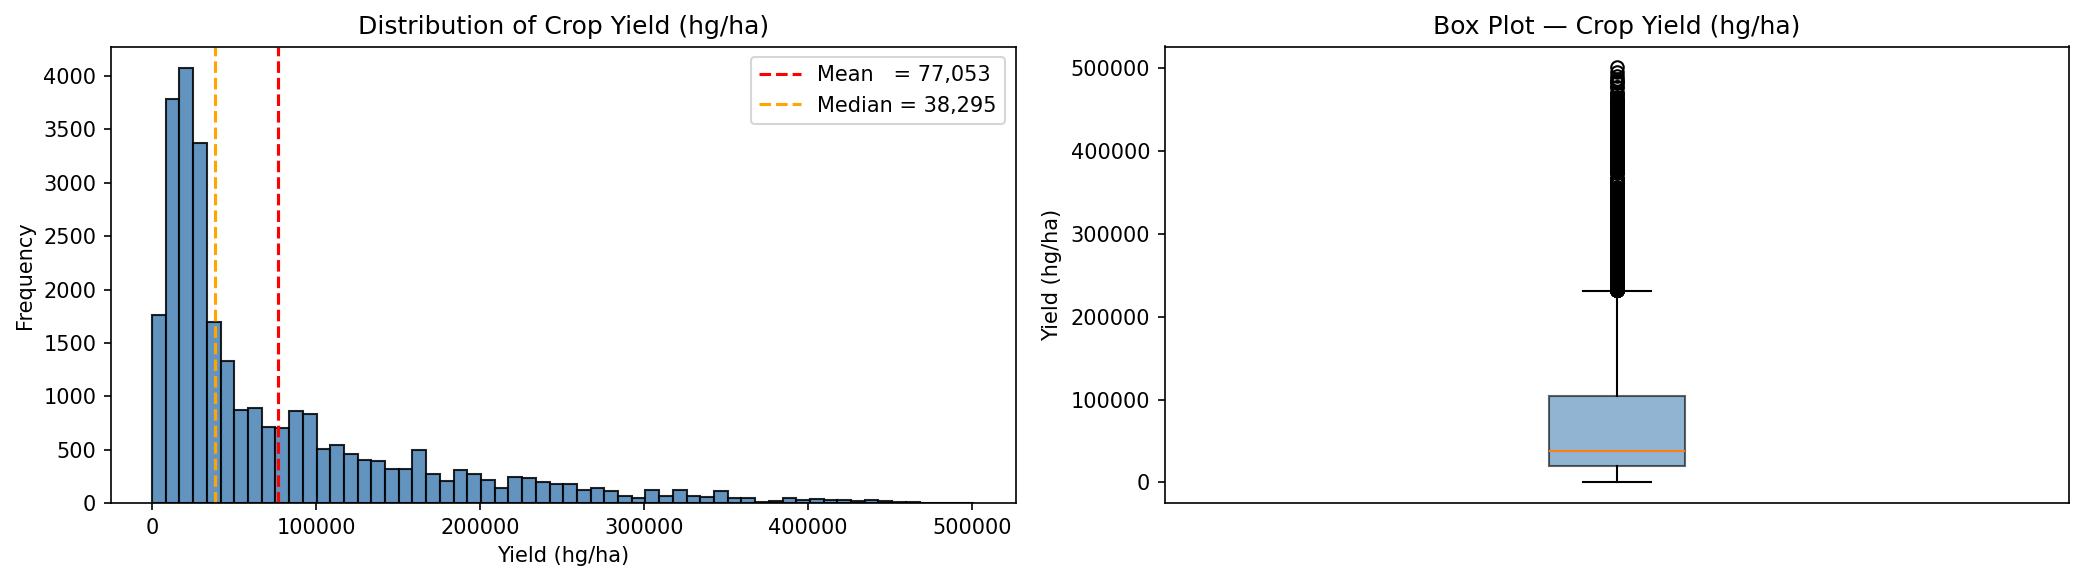
\includegraphics[width=\textwidth]{01_yield_distribution.png}
\caption{Distribution of crop yield (histogram and box plot). The distribution
is heavily right-skewed: most records sit at low yields, with a long tail of
high-yield crops.}
\end{figure}

\begin{figure}[H]
\centering
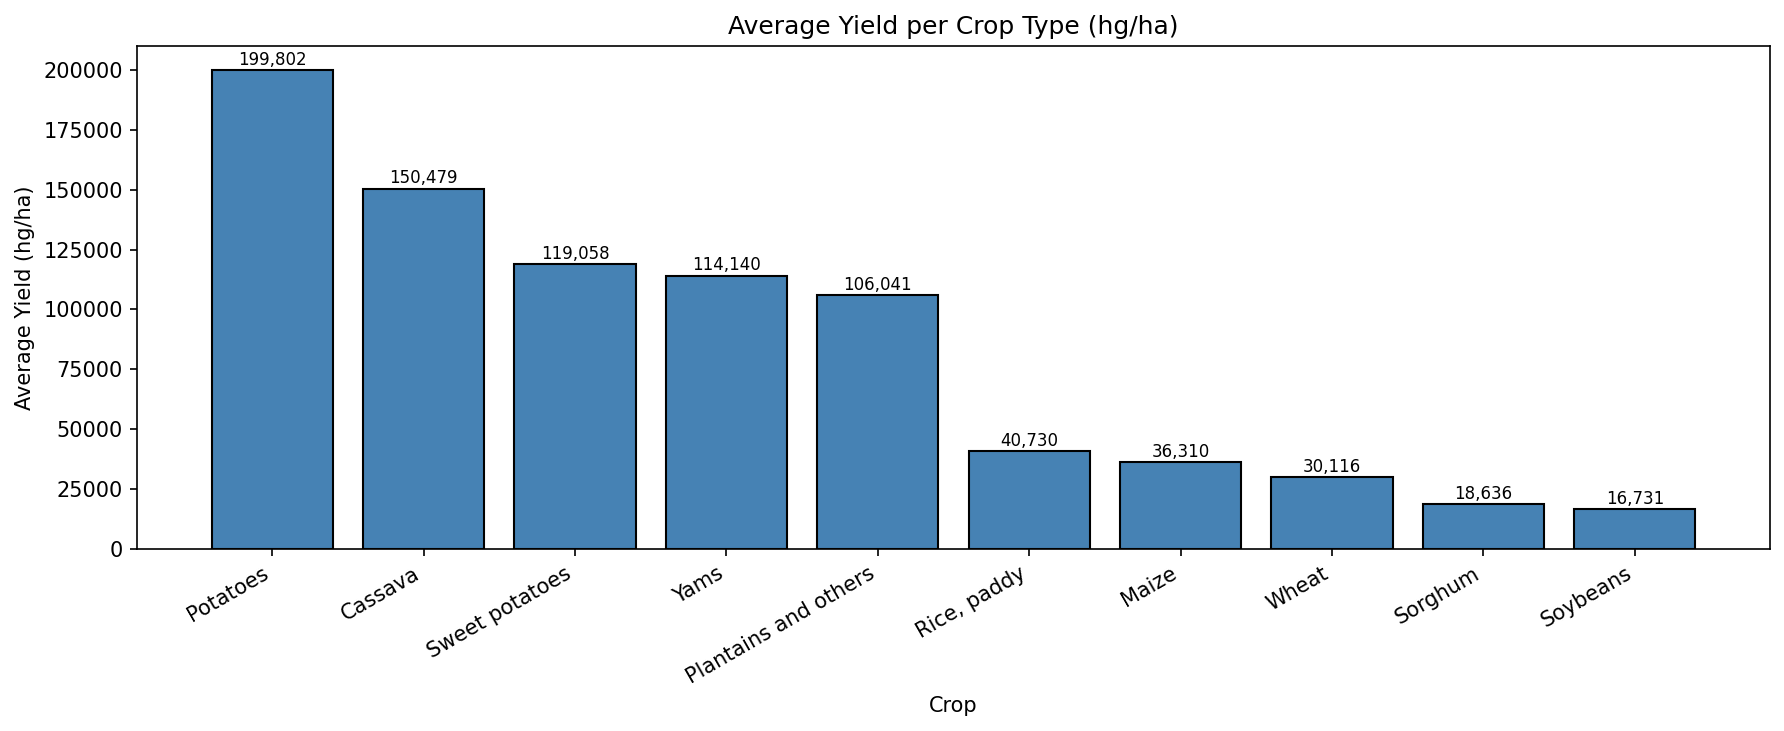
\includegraphics[width=0.85\textwidth]{02_avg_yield_per_crop.png}
\caption{Average yield per crop. Root crops such as Cassava and Potatoes yield
far more (hg/ha) than cereals such as Wheat and Sorghum, showing that the crop
type is a major driver of yield.}
\end{figure}

\begin{figure}[H]
\centering
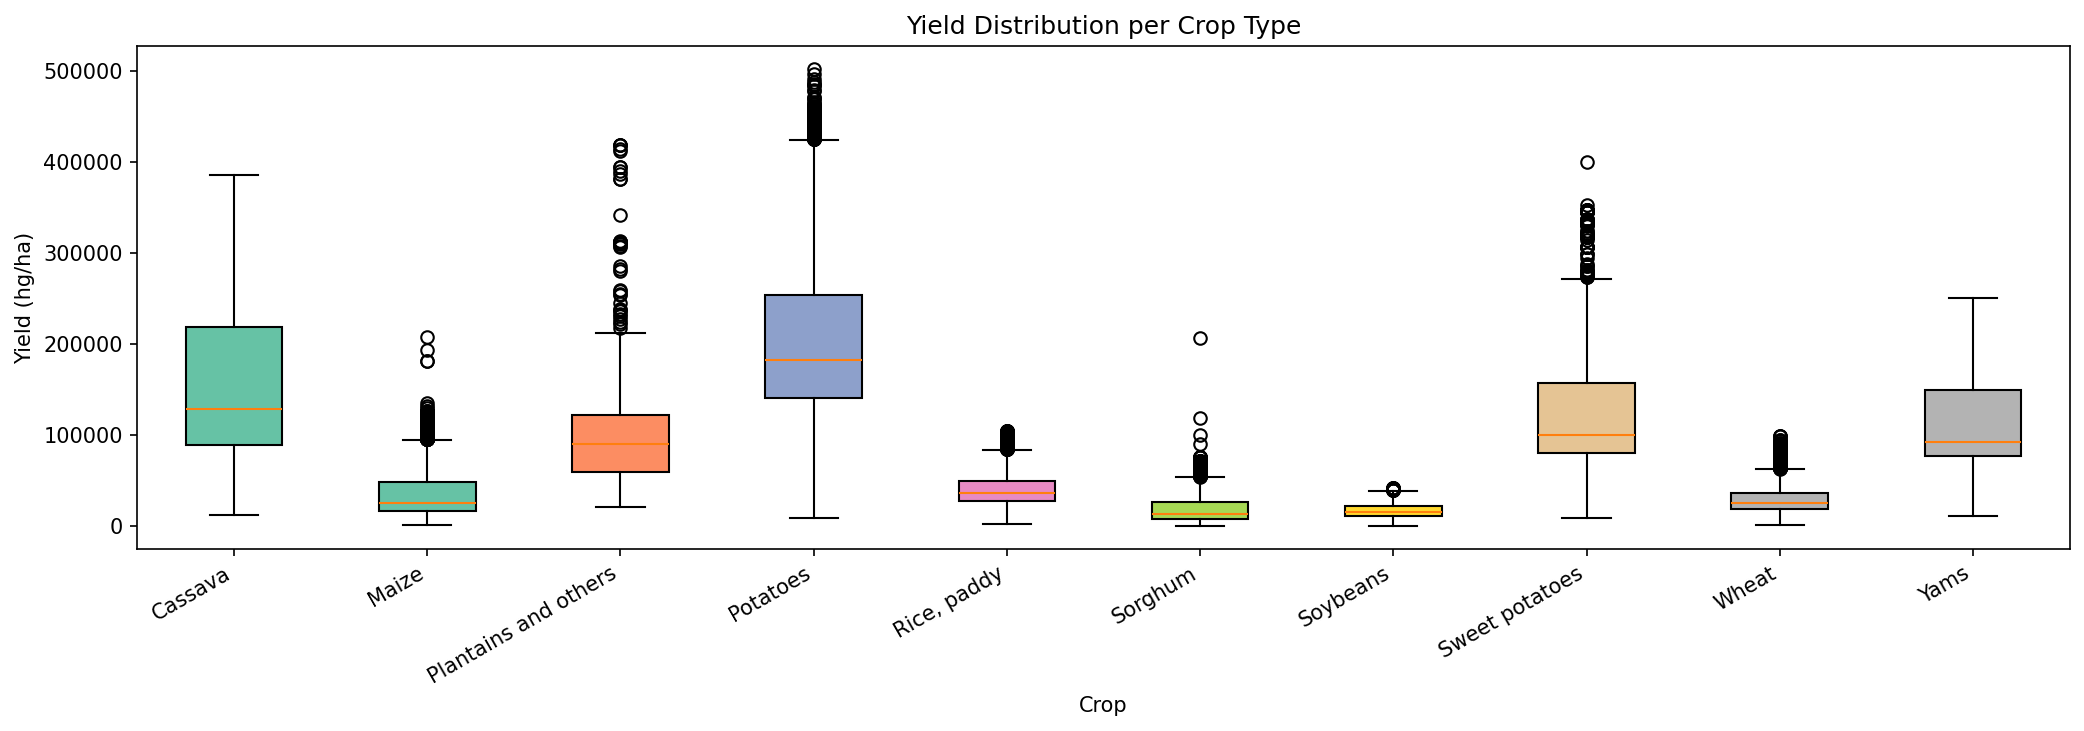
\includegraphics[width=\textwidth]{03_yield_boxplots_per_crop.png}
\caption{Yield distribution per crop (box plots), confirming both the
between-crop differences and the within-crop spread.}
\end{figure}

\begin{figure}[H]
\centering
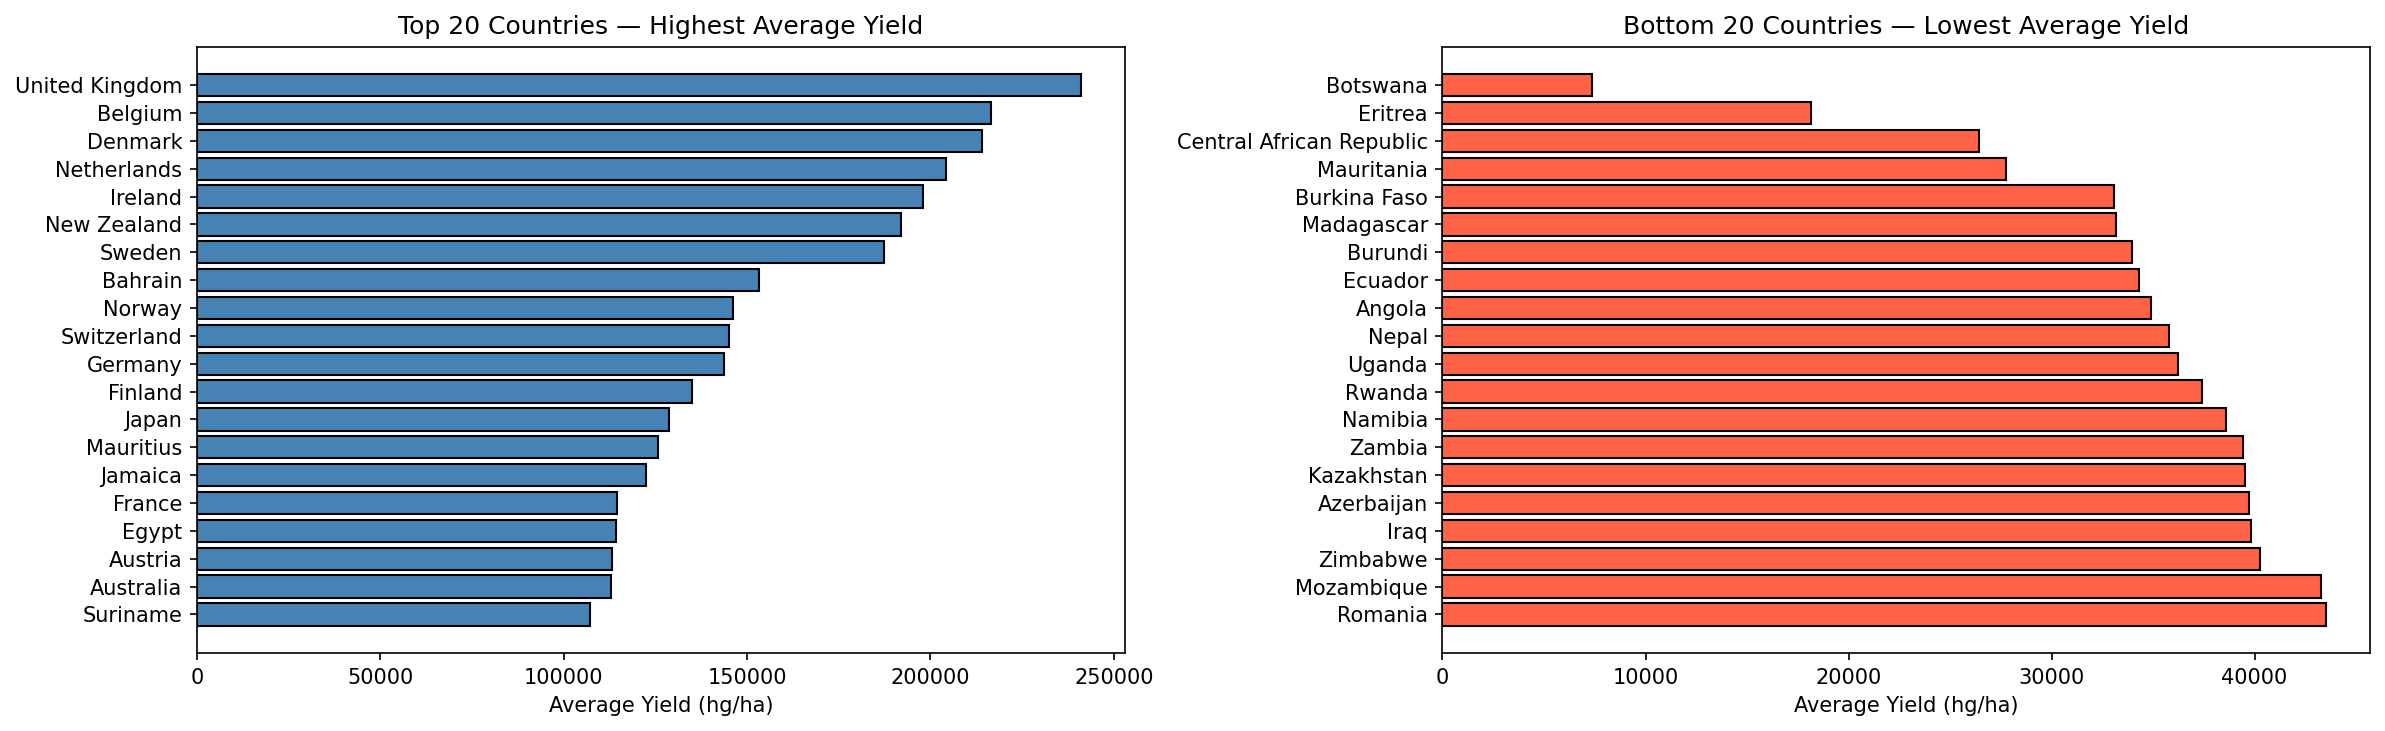
\includegraphics[width=0.9\textwidth]{04_top20_countries.png}
\caption{Top 20 countries by average yield. High-yield countries are
concentrated in regions with intensive agriculture.}
\end{figure}

\begin{figure}[H]
\centering
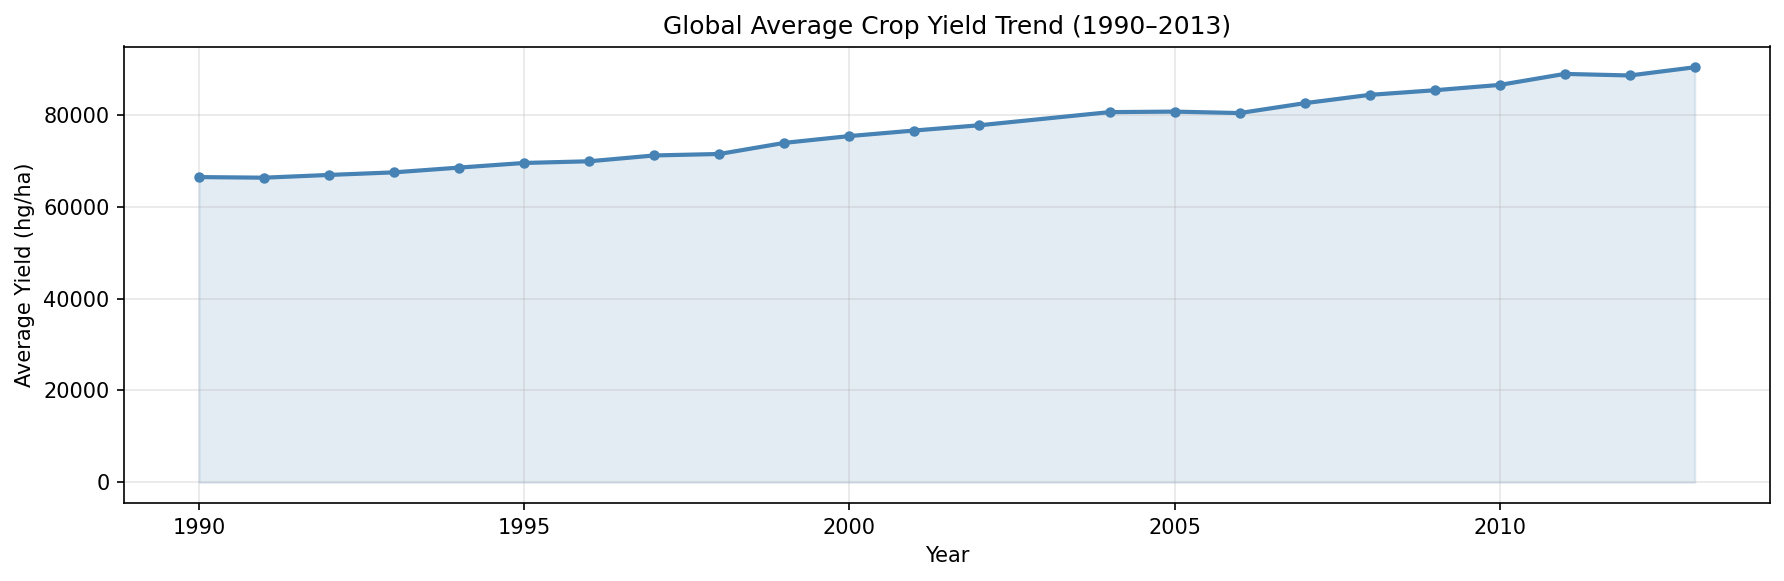
\includegraphics[width=0.85\textwidth]{05_yield_trend_years.png}
\caption{Global average yield trend over time (1990--2013), showing a gradual
upward trend.}
\end{figure}

\begin{figure}[H]
\centering
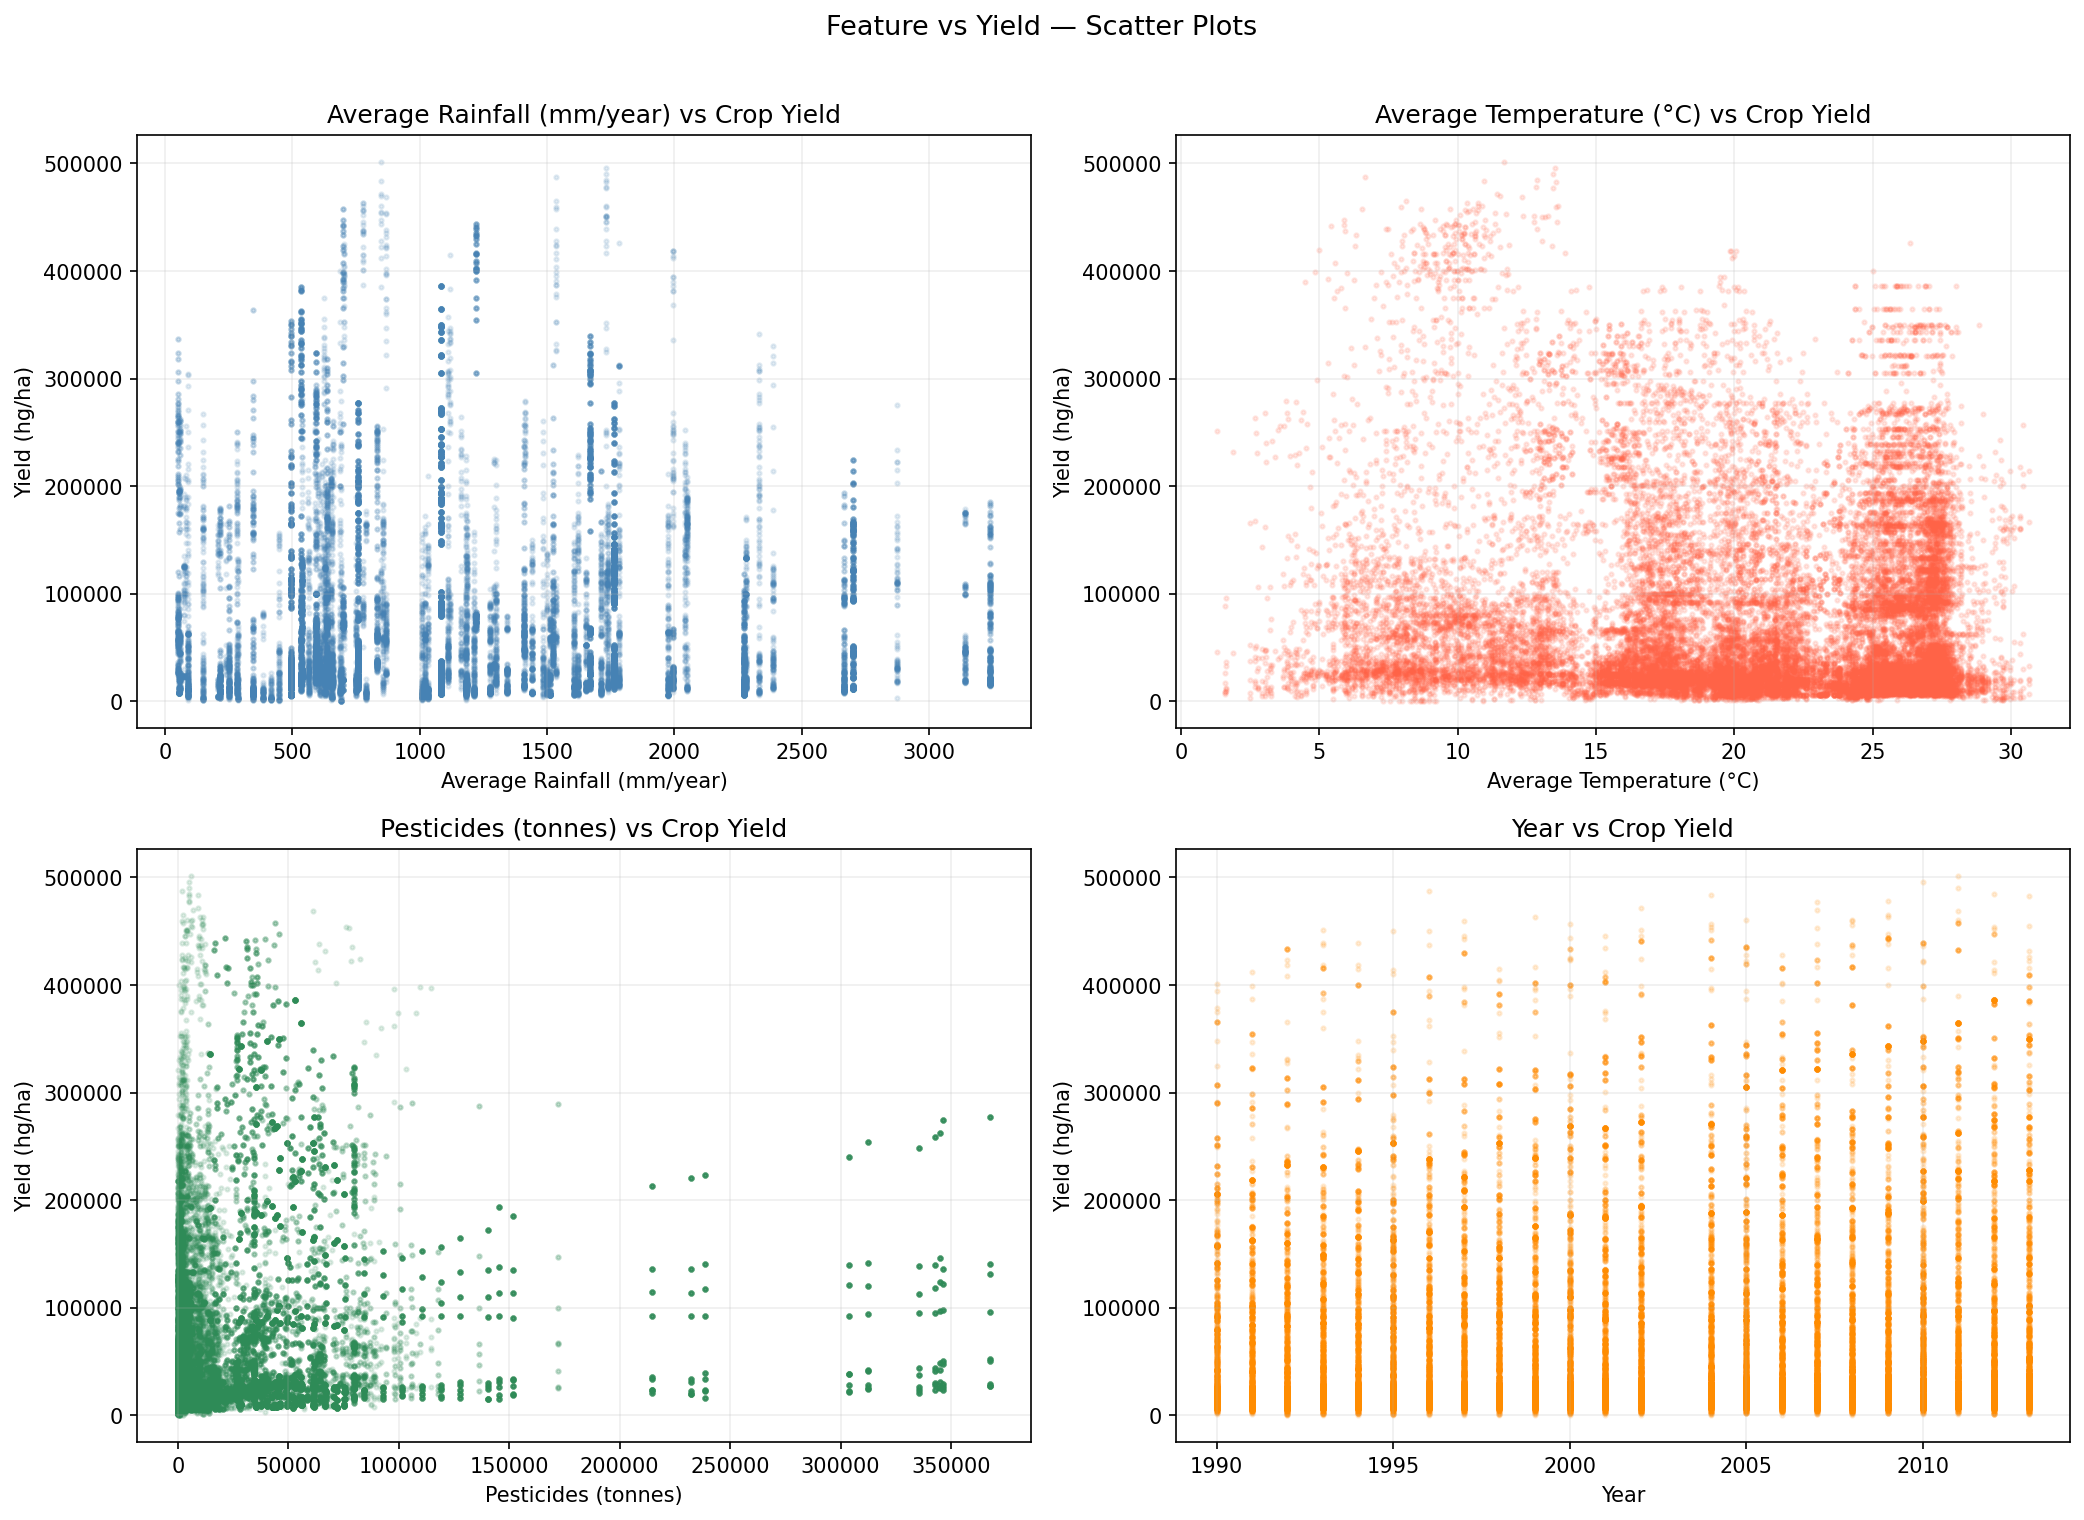
\includegraphics[width=\textwidth]{06_feature_vs_target_scatter.png}
\caption{Scatter plots of each numerical feature against yield. The
relationships are weak and non-linear, suggesting that linear models alone will
be insufficient.}
\end{figure}

\begin{figure}[H]
\centering
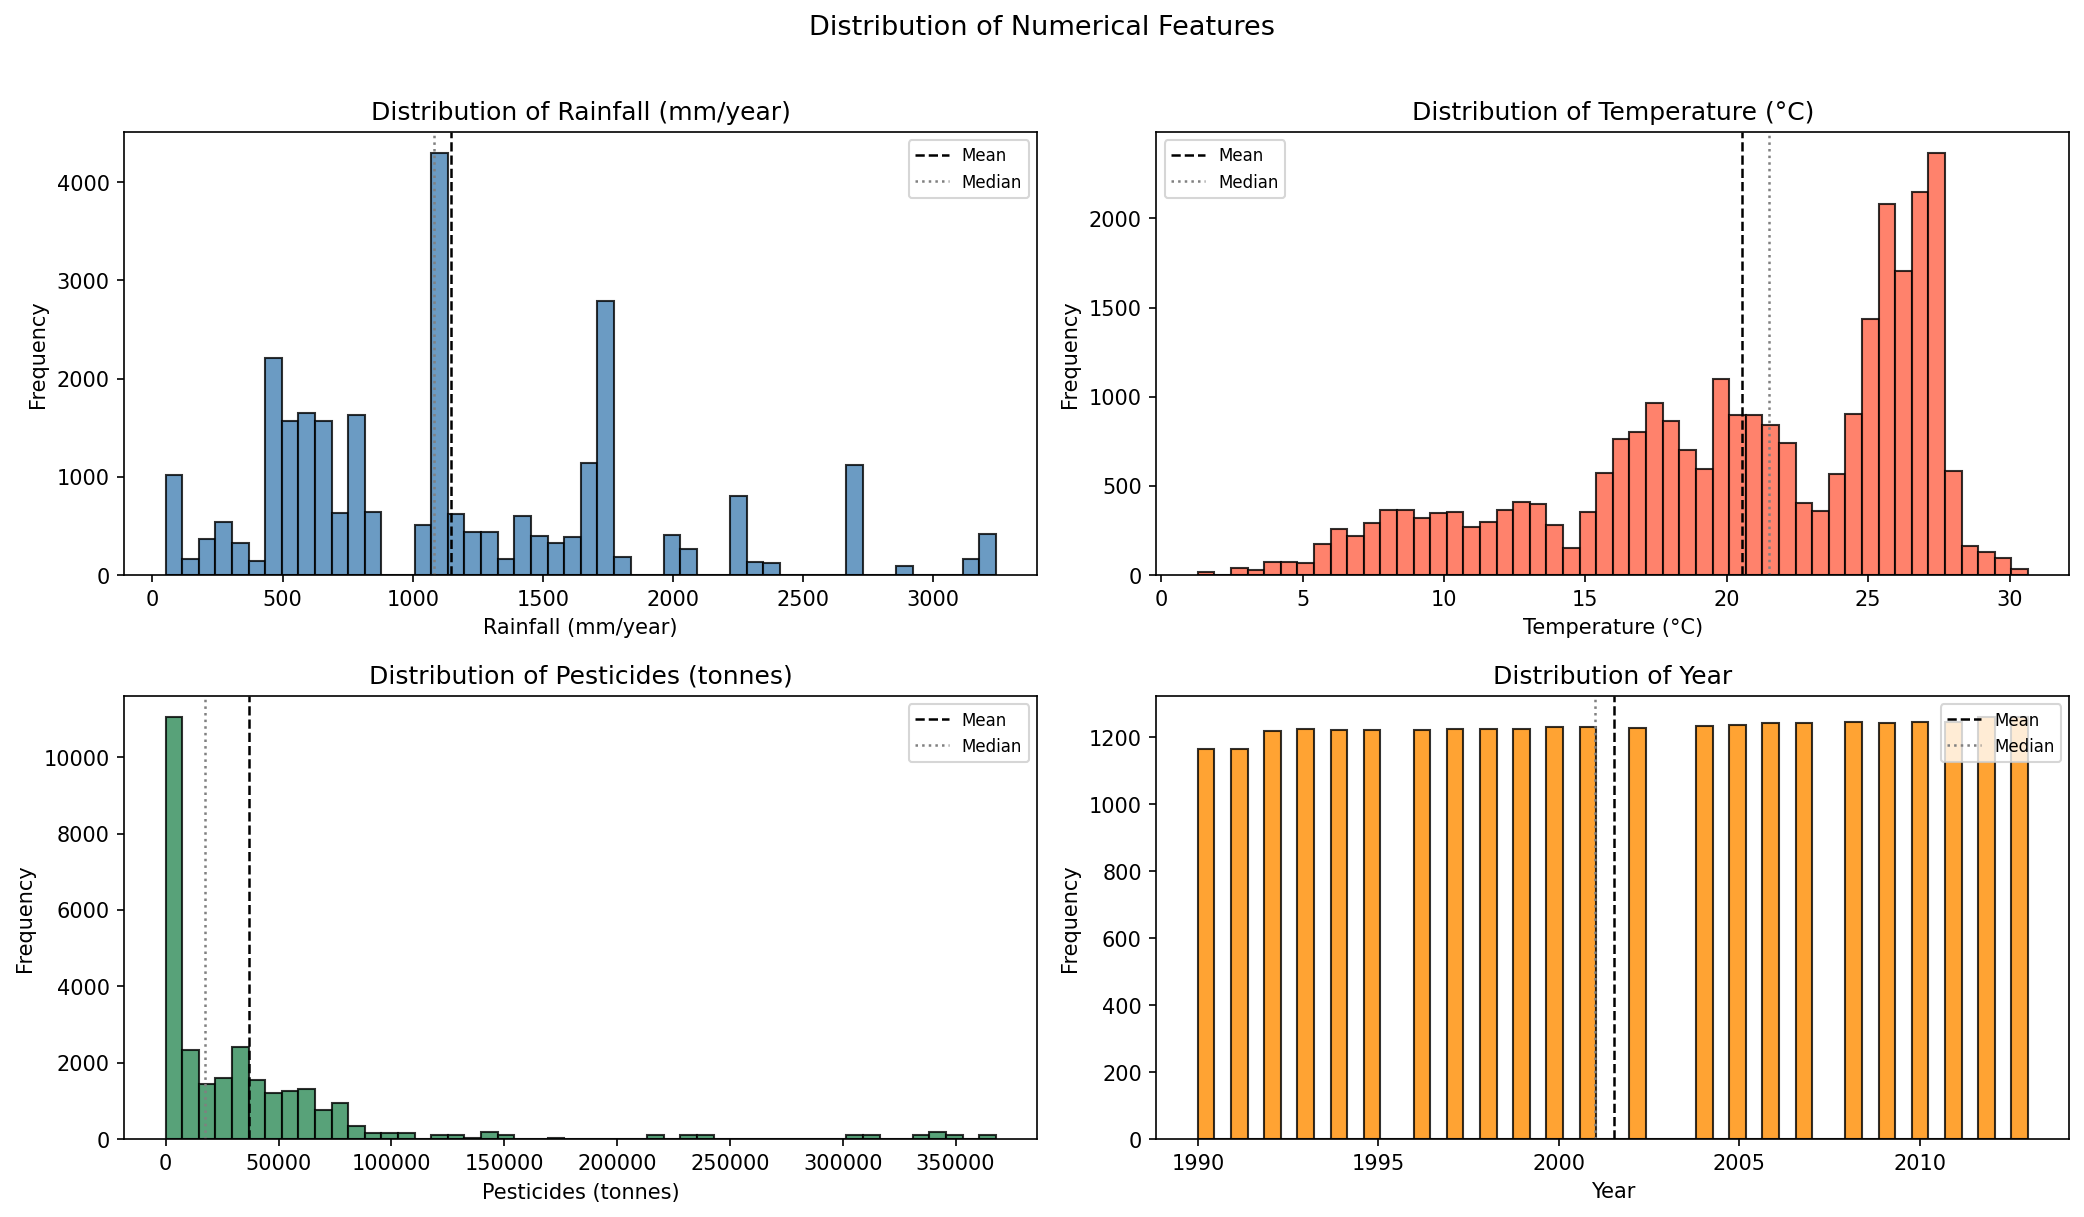
\includegraphics[width=\textwidth]{07_numeric_feature_distributions.png}
\caption{Distributions of the four numerical features.}
\end{figure}

\begin{figure}[H]
\centering
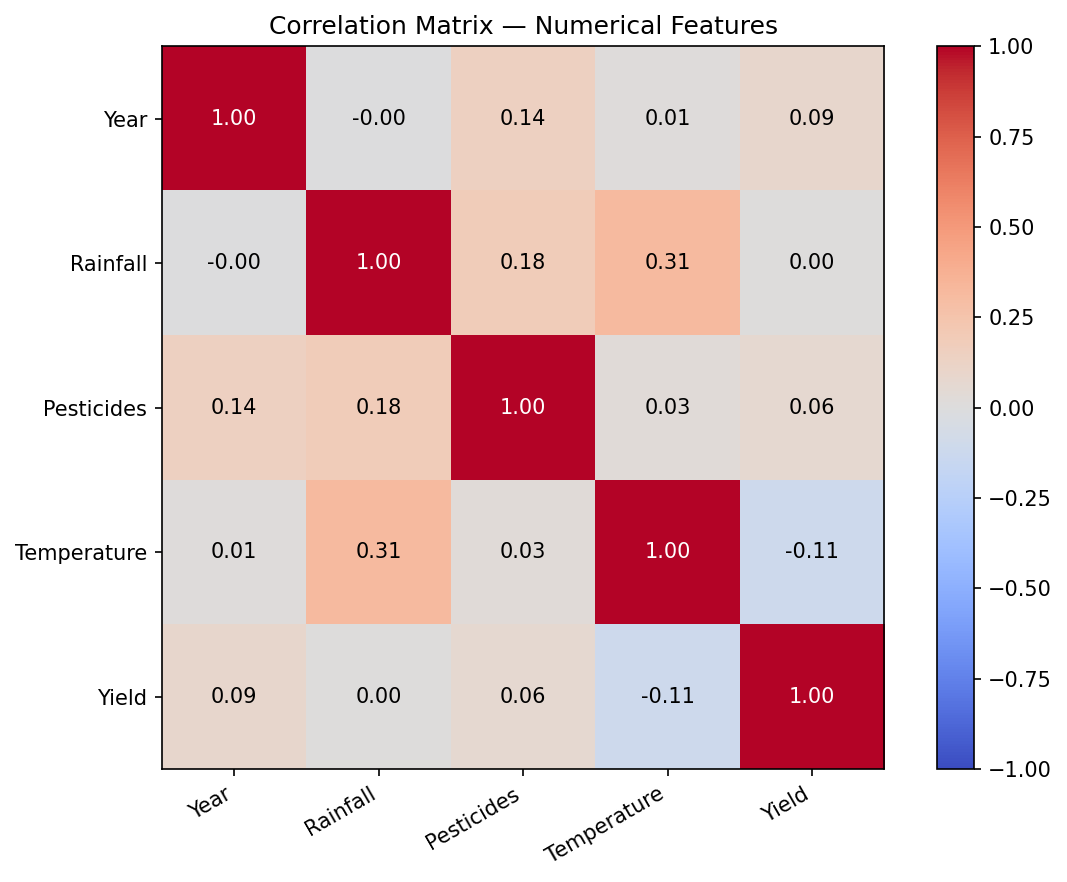
\includegraphics[width=0.7\textwidth]{08_correlation_heatmap.png}
\caption{Correlation between the numerical features and yield. The numerical
features are only weakly correlated with the target (temperature $-0.11$,
pesticides $+0.06$, rainfall $\approx 0$).}
\end{figure}

\paragraph{Key observations.}
\begin{itemize}[noitemsep]
  \item The yield distribution is strongly right-skewed.
  \item Crop type (and country) explain far more of the variance than the
        numerical climate features, whose linear correlation with yield is weak.
  \item There are no missing values, so no imputation is required.
  \item The weak, non-linear numeric relationships indicate that non-linear
        ensemble models should outperform linear ones.
\end{itemize}

% ================================================================ 4
\section{Data Preprocessing}\label{sec:prep}

The same preprocessing pipeline is used for both tasks:

\begin{enumerate}[noitemsep]
  \item \textbf{Drop the index column} and split the six input columns from the
        target \texttt{hg/ha\_yield}.
  \item \textbf{One-hot encode} the two categorical columns: \texttt{Area}
        (101 countries) and \texttt{Item} (10 crops), producing 111 binary
        columns.
  \item Keep the four numerical columns unchanged, giving a total of
        \textbf{115 model features}.
  \item \textbf{Scale} only the four numerical columns with a
        \texttt{StandardScaler}, fit on the \emph{training set only} to prevent
        data leakage. The 111 binary columns are left as-is.
  \item \textbf{Split} into train/test: 80/20 for regression and 75/25 for
        classification (\texttt{random\_state=0}).
\end{enumerate}

The feature expansion is the central preprocessing step:
\[
\underbrace{101}_{\text{Area}} \;+\; \underbrace{10}_{\text{Item}}
\;=\; 111 \text{ one-hot columns} \;+\; 4 \text{ numeric columns}
\;=\; \boxed{115 \text{ features}}.
\]
The six original columns therefore become 115 features fed into every model.
For polynomial regression, \texttt{PolynomialFeatures} is applied only to the
four numerical columns (to avoid an explosion from the 111 binary columns) and
then concatenated back with the one-hot columns.

% ================================================================ 5
\section{Regression Models and Results}\label{sec:reg}

Six regression models were trained, plus a naive mean-predictor baseline:
Linear Regression, Polynomial Regression (degrees 2 and 3), Decision Tree,
Random Forest, Gradient Boosting, and Support Vector Regression (SVR, RBF
kernel).

\begin{table}[H]
\centering
\caption{Regression benchmark on the held-out test set. Random Forest is the
best model; SVR performs worse than the baseline.}
\begin{tabular}{lrrr}
\toprule
\textbf{Model} & \textbf{$R^2$} & \textbf{MAE} & \textbf{RMSE} \\
\midrule
\textbf{Random Forest}      & \textbf{0.9888} & 3{,}494  & 9{,}143  \\
Decision Tree               & 0.9823 & 3{,}607  & 11{,}508 \\
Gradient Boosting           & 0.8718 & 19{,}912 & 30{,}952 \\
Polynomial (deg=3)          & 0.7600 & 29{,}389 & 42{,}345 \\
Polynomial (deg=2)          & 0.7598 & 29{,}369 & 42{,}364 \\
Linear Regression           & 0.7597 & 29{,}261 & 42{,}368 \\
Baseline (mean)             & $-0.0003$ & 65{,}021 & 86{,}449 \\
SVR (RBF)                   & $-0.2121$ & 58{,}168 & 95{,}162 \\
\bottomrule
\end{tabular}
\end{table}

\begin{figure}[H]
\centering
\begin{subfigure}{0.49\textwidth}
  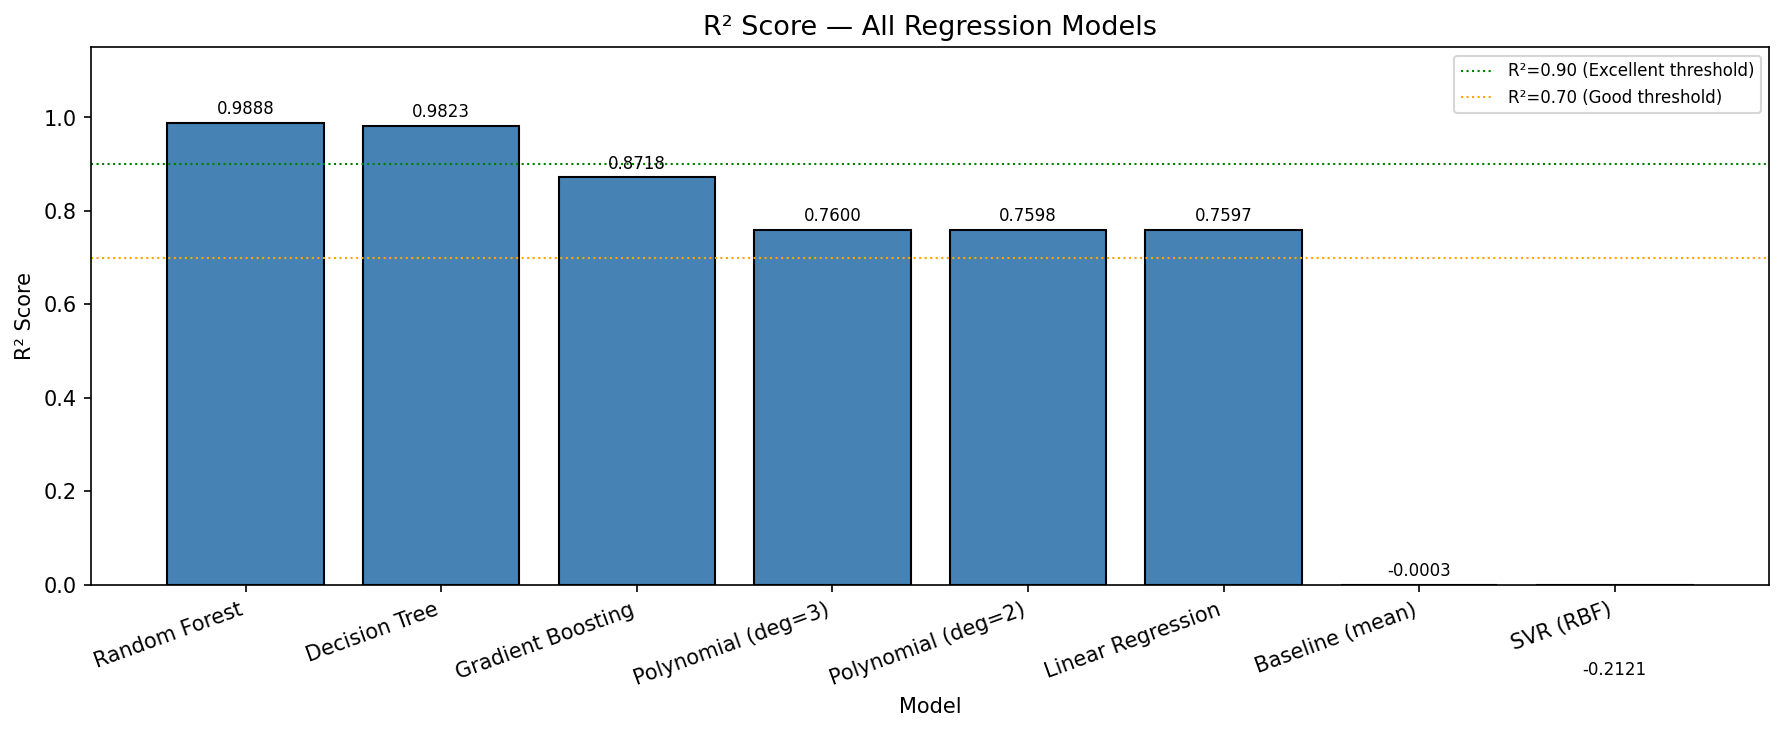
\includegraphics[width=\textwidth]{18_r2_comparison.png}
  \caption{$R^2$ score (higher is better).}
\end{subfigure}\hfill
\begin{subfigure}{0.49\textwidth}
  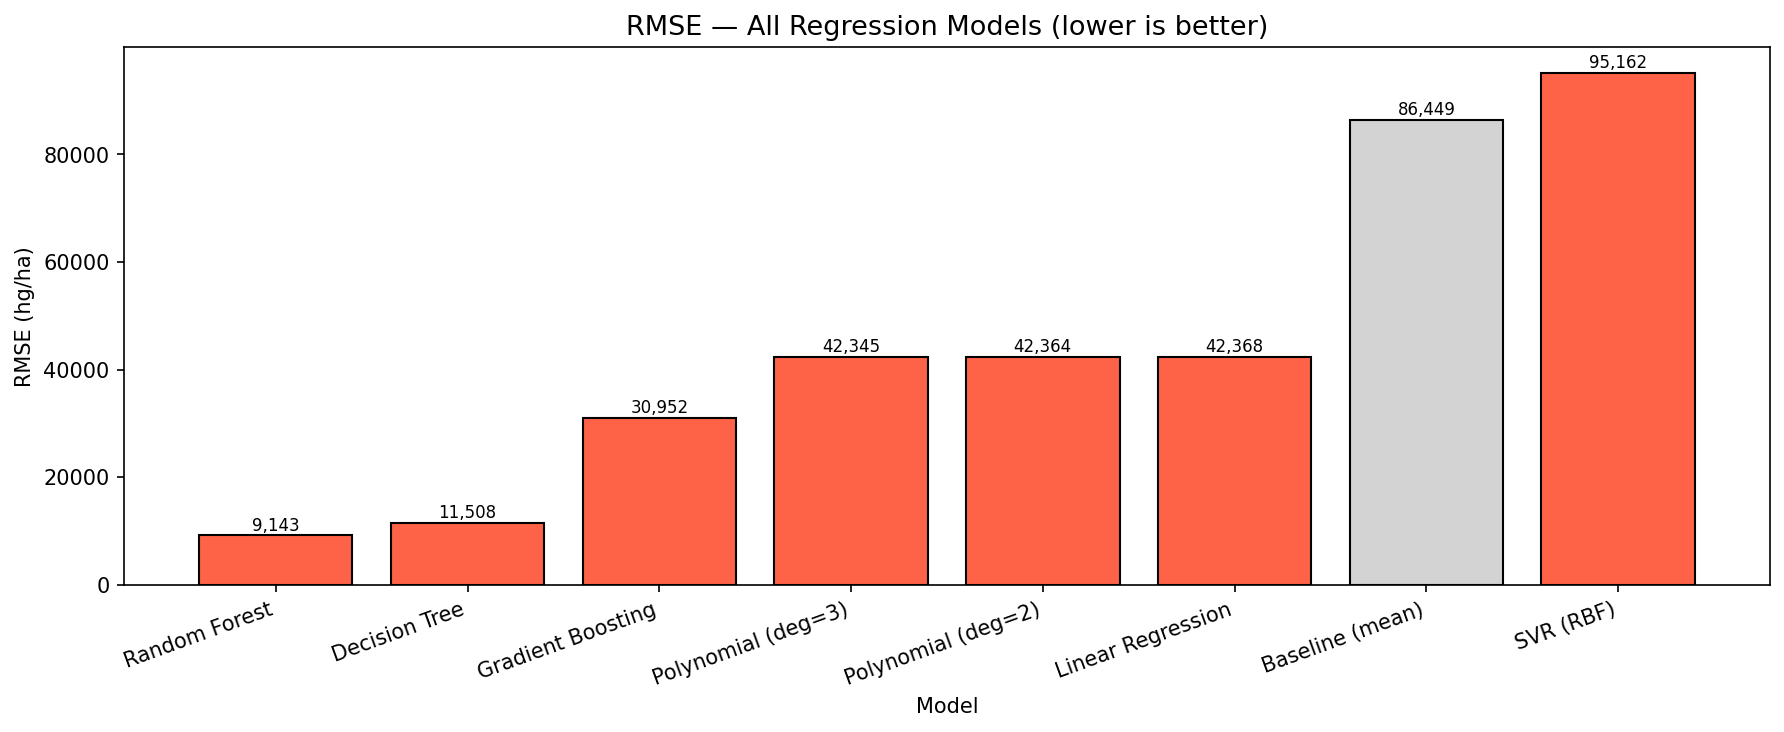
\includegraphics[width=\textwidth]{19_rmse_comparison.png}
  \caption{RMSE (lower is better).}
\end{subfigure}
\caption{Regression model comparison. Ensemble tree models clearly dominate the
linear and polynomial models.}
\end{figure}

\begin{figure}[H]
\centering
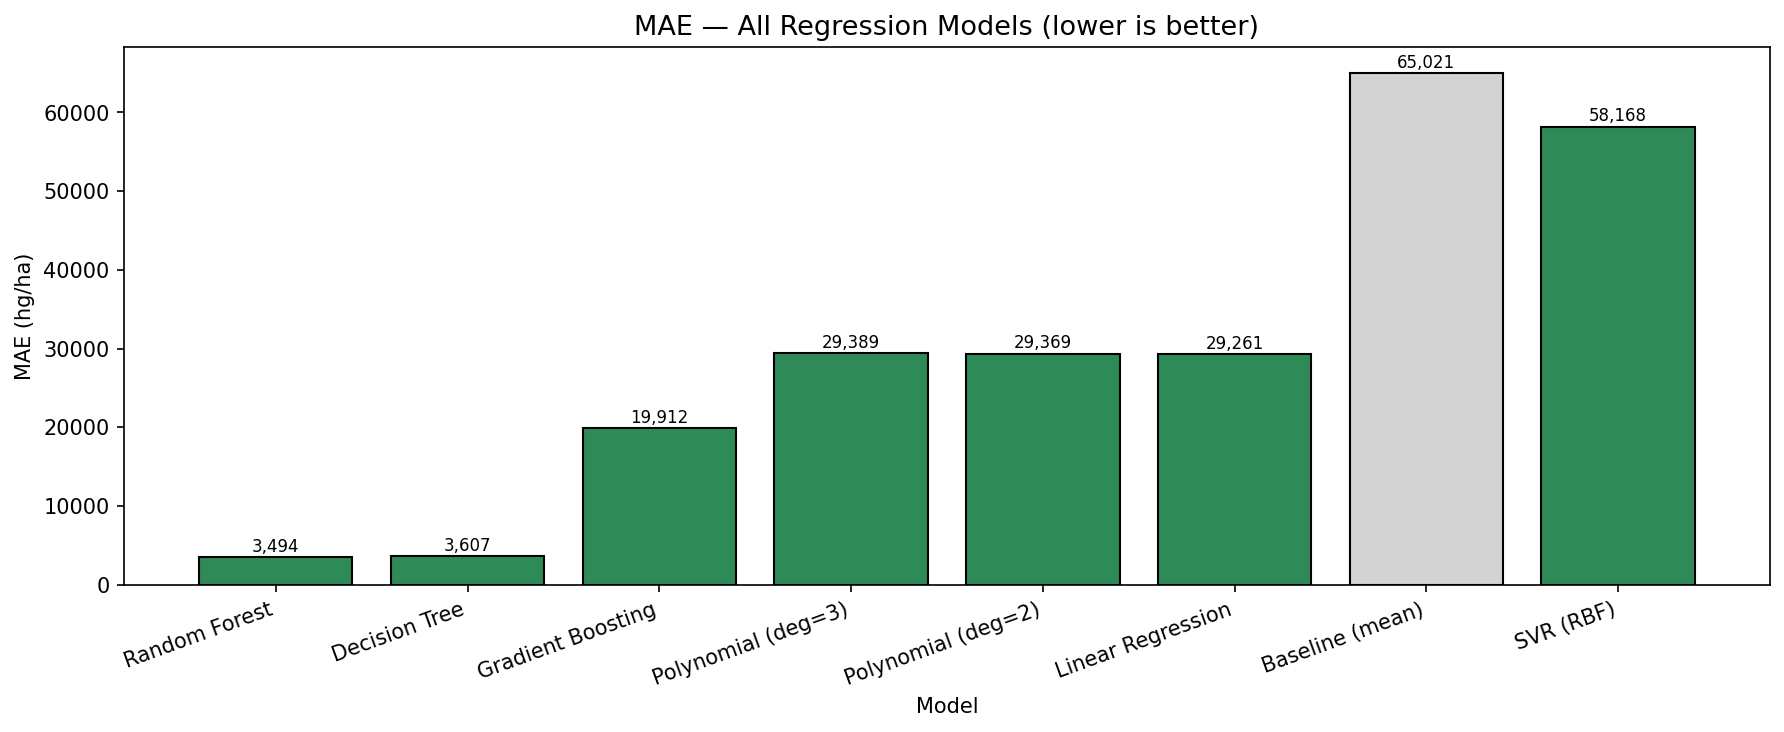
\includegraphics[width=0.9\textwidth]{20_mae_comparison.png}
\caption{Mean Absolute Error (MAE) by model (lower is better).}
\end{figure}

\begin{figure}[H]
\centering
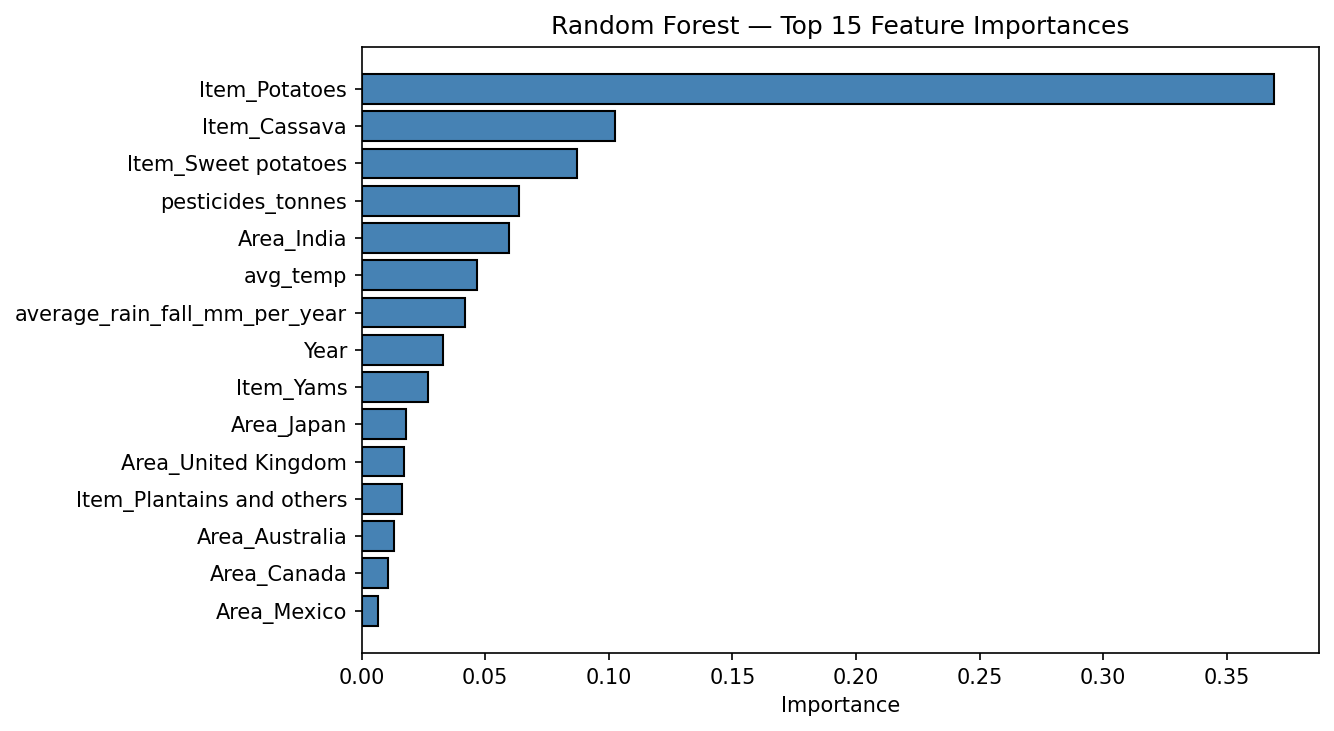
\includegraphics[width=0.85\textwidth]{14_feature_importance_rf.png}
\caption{Random Forest feature importance (top 15). Pesticide use, year, and the
climate features, together with a few dominant crop types, drive predictions.}
\end{figure}

\begin{figure}[H]
\centering
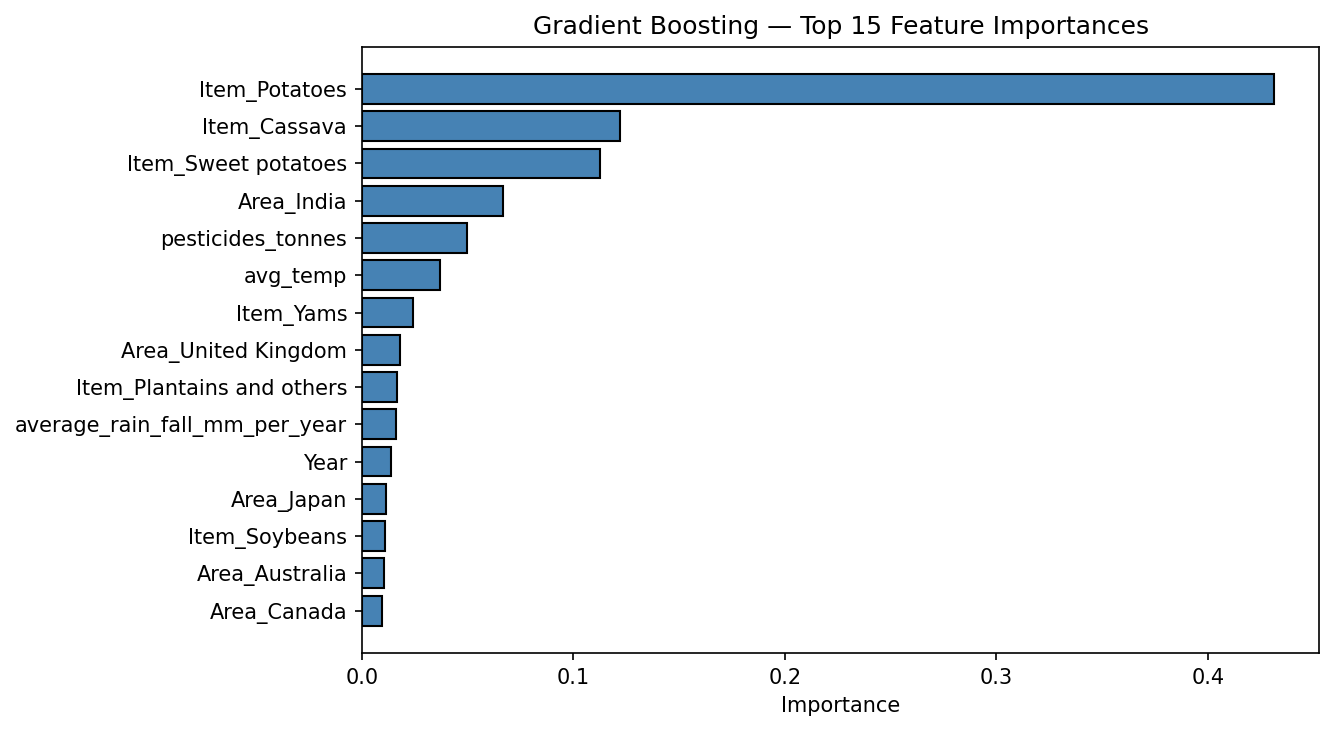
\includegraphics[width=0.85\textwidth]{16_feature_importance_gb.png}
\caption{Gradient Boosting feature importance (top 15).}
\end{figure}

\begin{figure}[H]
\centering
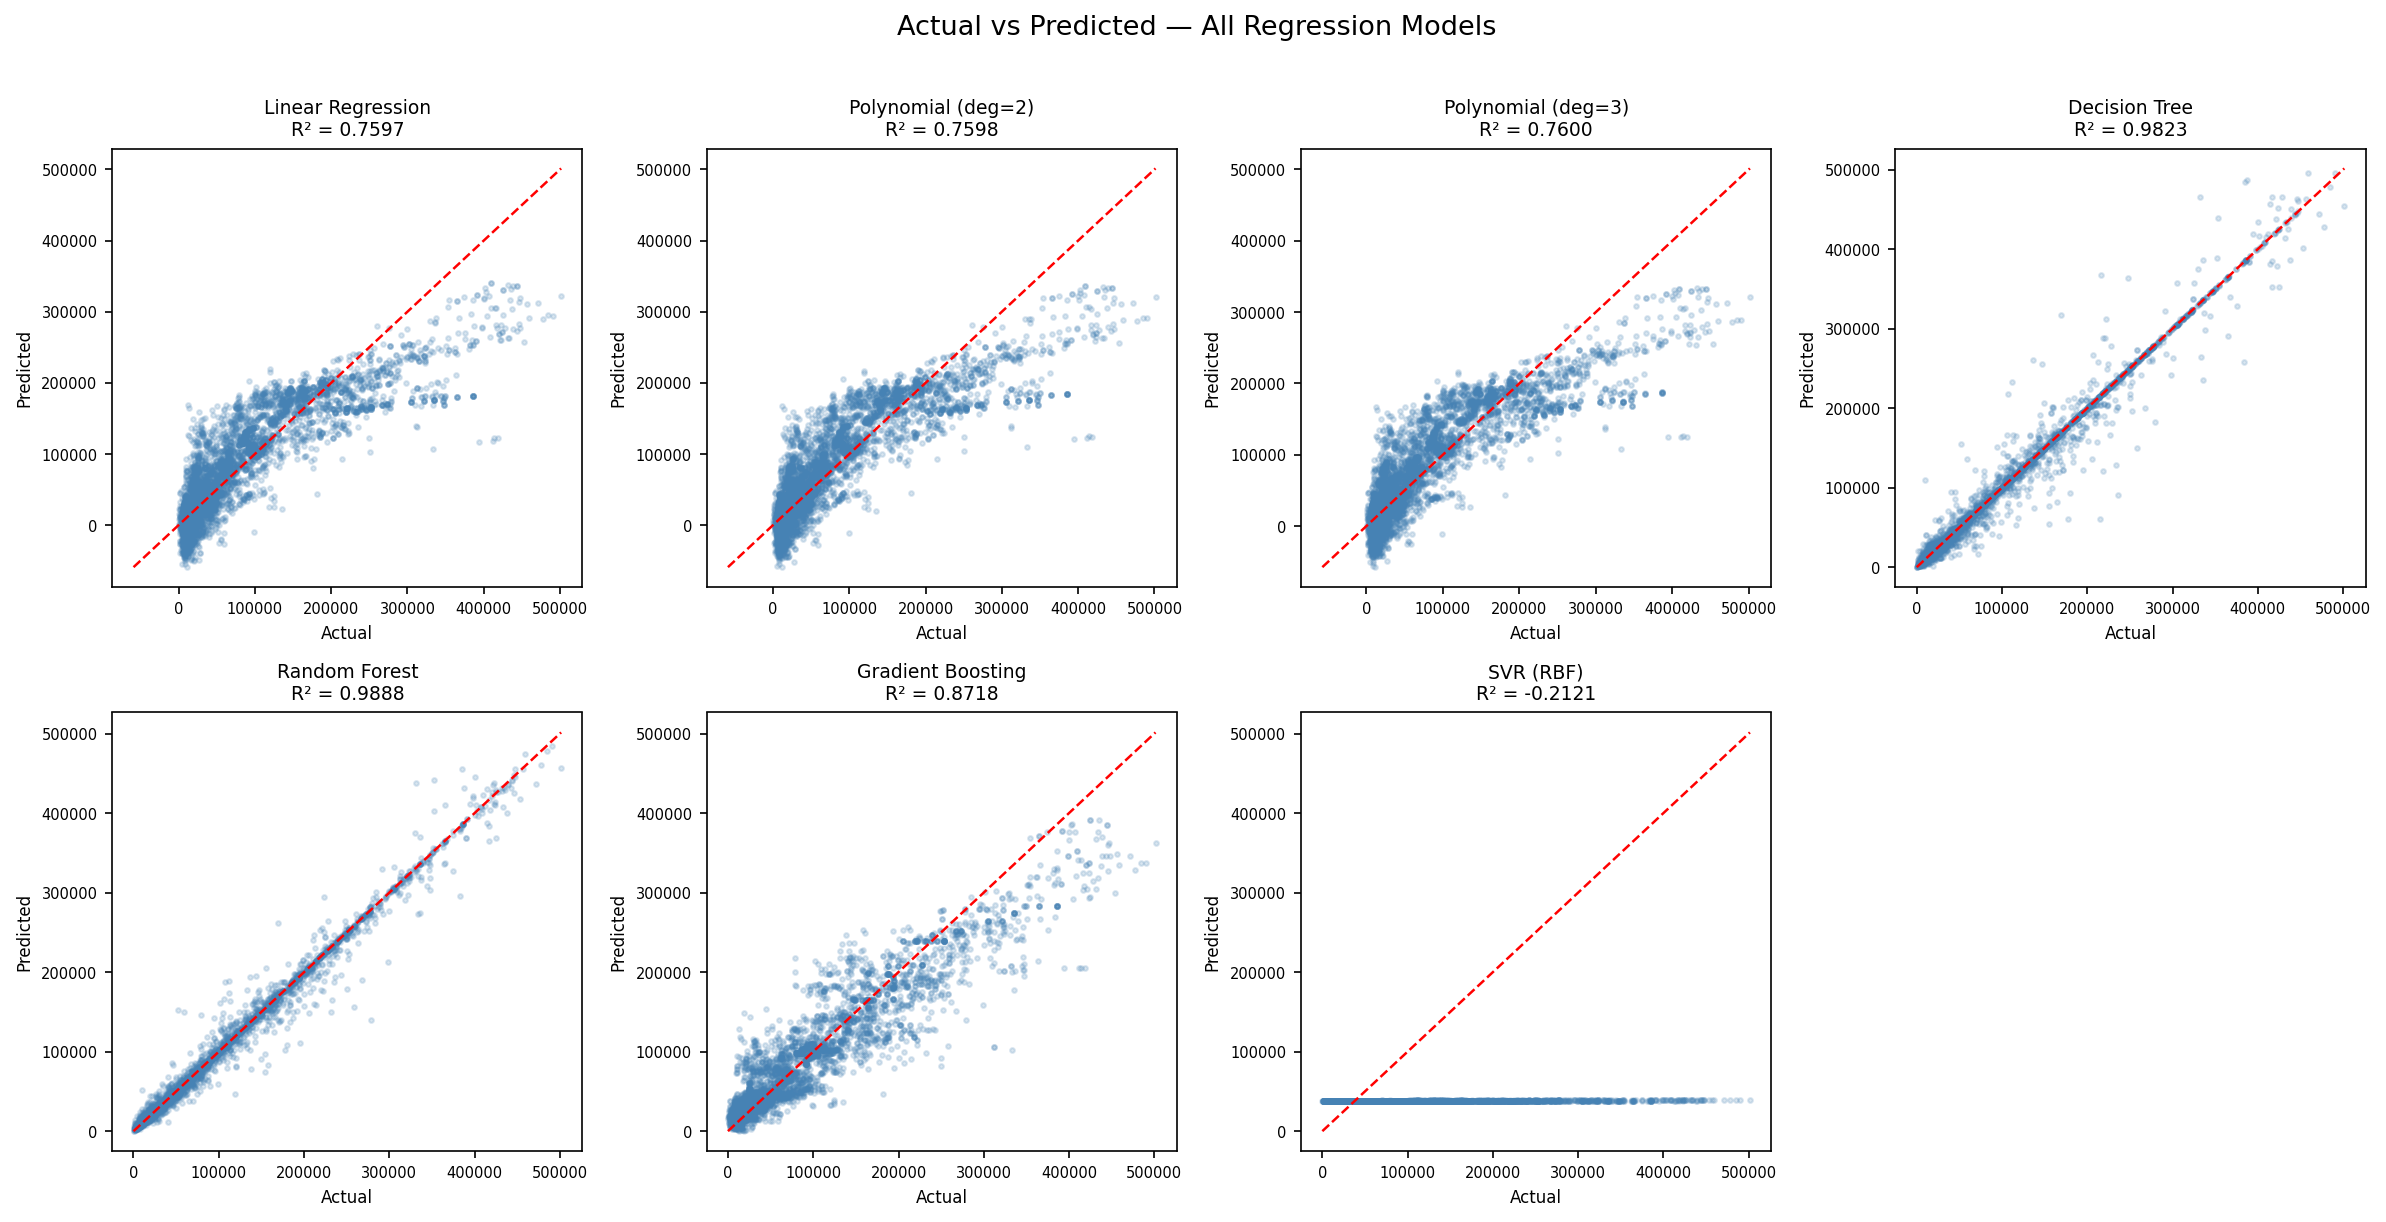
\includegraphics[width=\textwidth]{21_actual_vs_predicted_all.png}
\caption{Actual vs.\ predicted yield for all models, side by side. The tighter
the points cluster on the diagonal, the better the model.}
\end{figure}

\paragraph{Per-model actual-vs-predicted and residual plots.}
The following figures show the diagnostic plots for each individual regression
model.

\begin{figure}[H]
\centering
\begin{subfigure}{0.49\textwidth}
  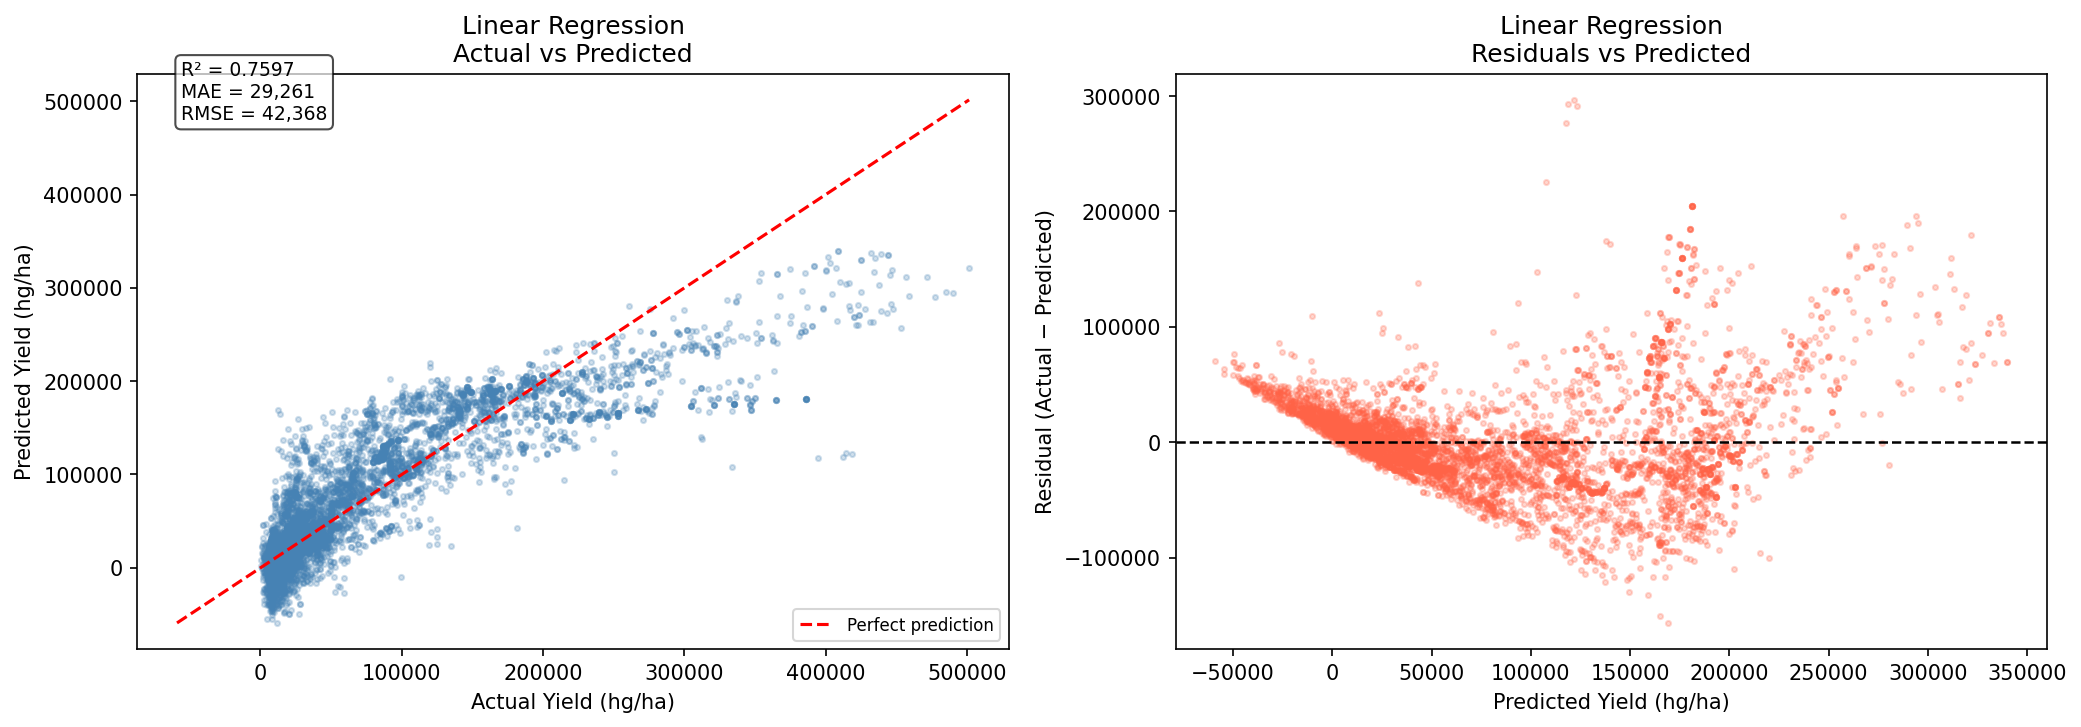
\includegraphics[width=\textwidth]{09_avp_linear_regression.png}
  \caption{Linear Regression.}
\end{subfigure}\hfill
\begin{subfigure}{0.49\textwidth}
  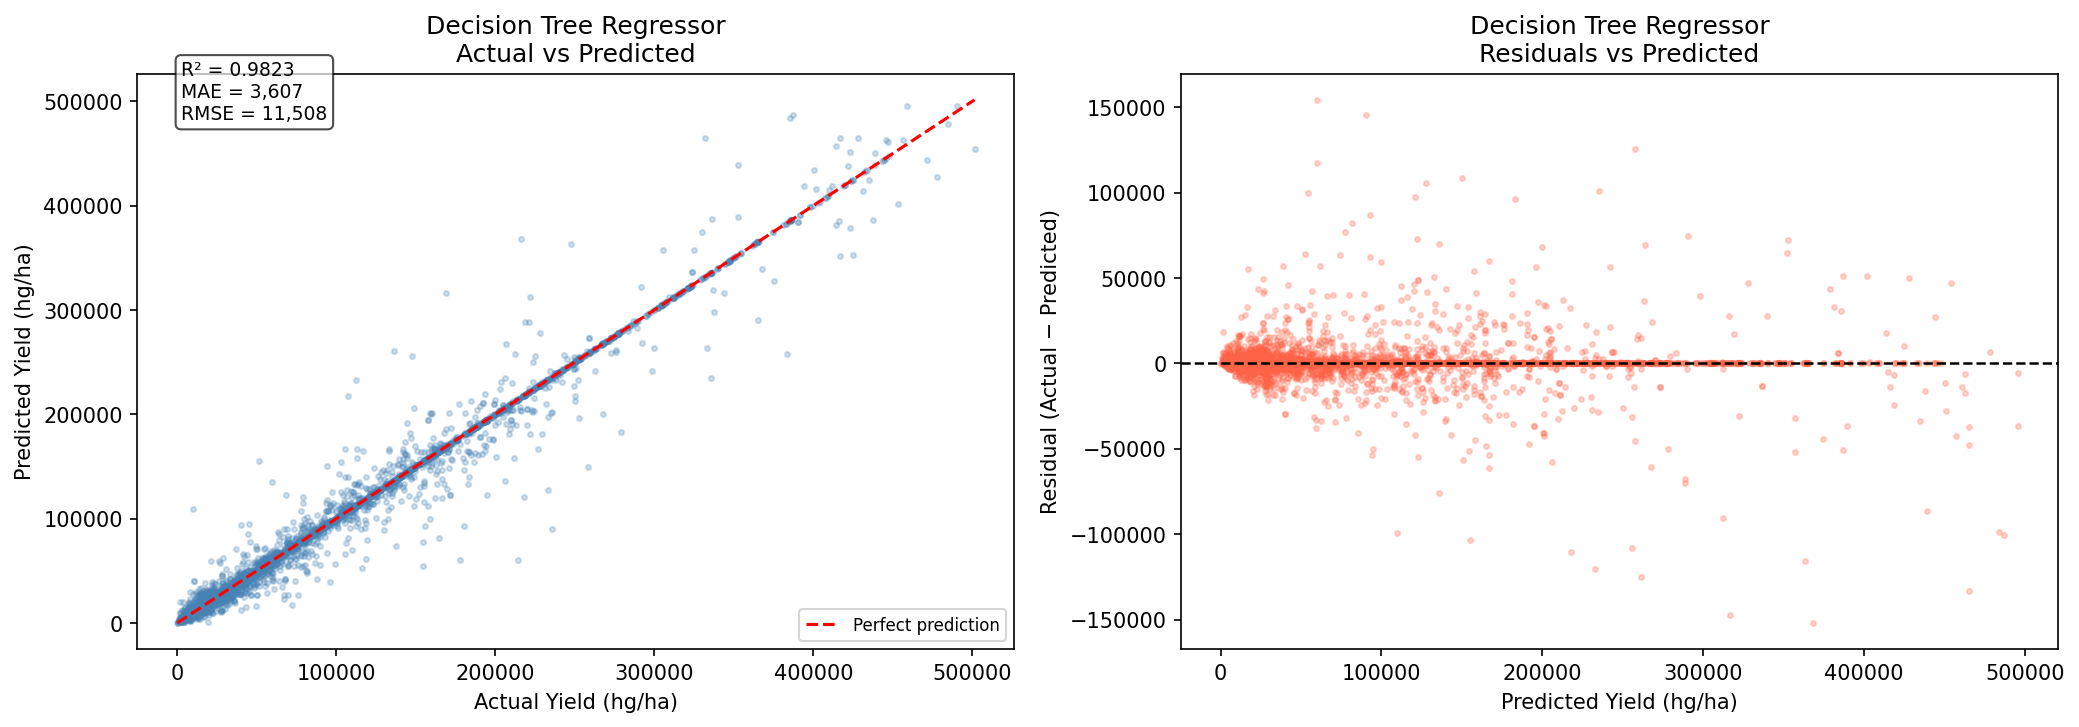
\includegraphics[width=\textwidth]{12_avp_decision_tree.png}
  \caption{Decision Tree.}
\end{subfigure}

\vspace{4pt}
\begin{subfigure}{0.49\textwidth}
  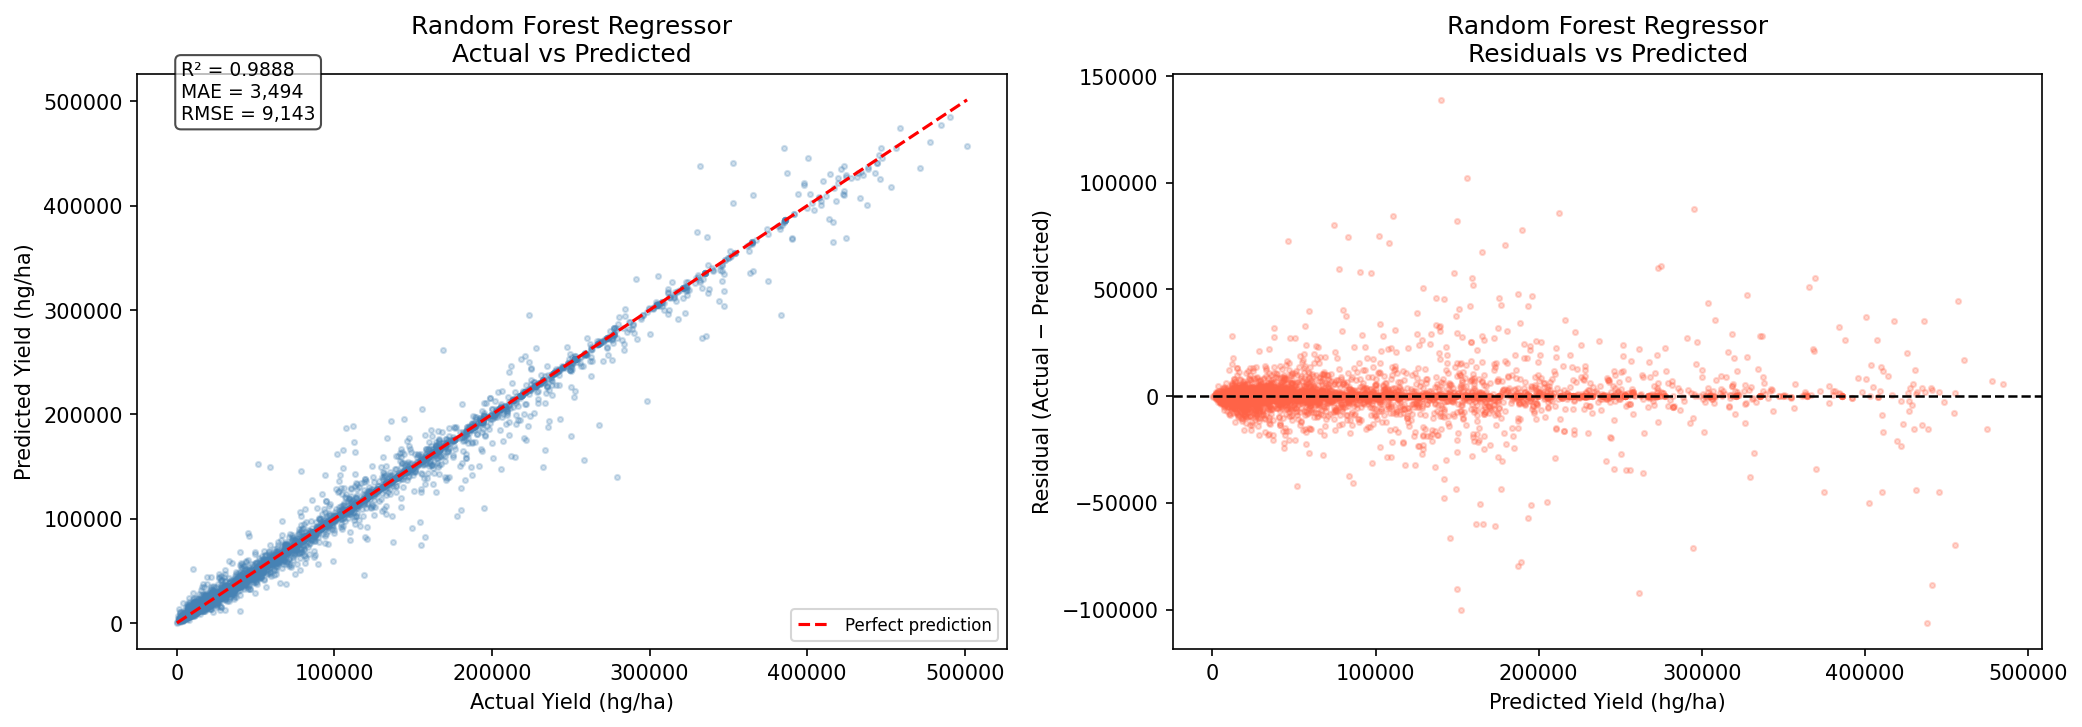
\includegraphics[width=\textwidth]{13_avp_random_forest.png}
  \caption{Random Forest (best).}
\end{subfigure}\hfill
\begin{subfigure}{0.49\textwidth}
  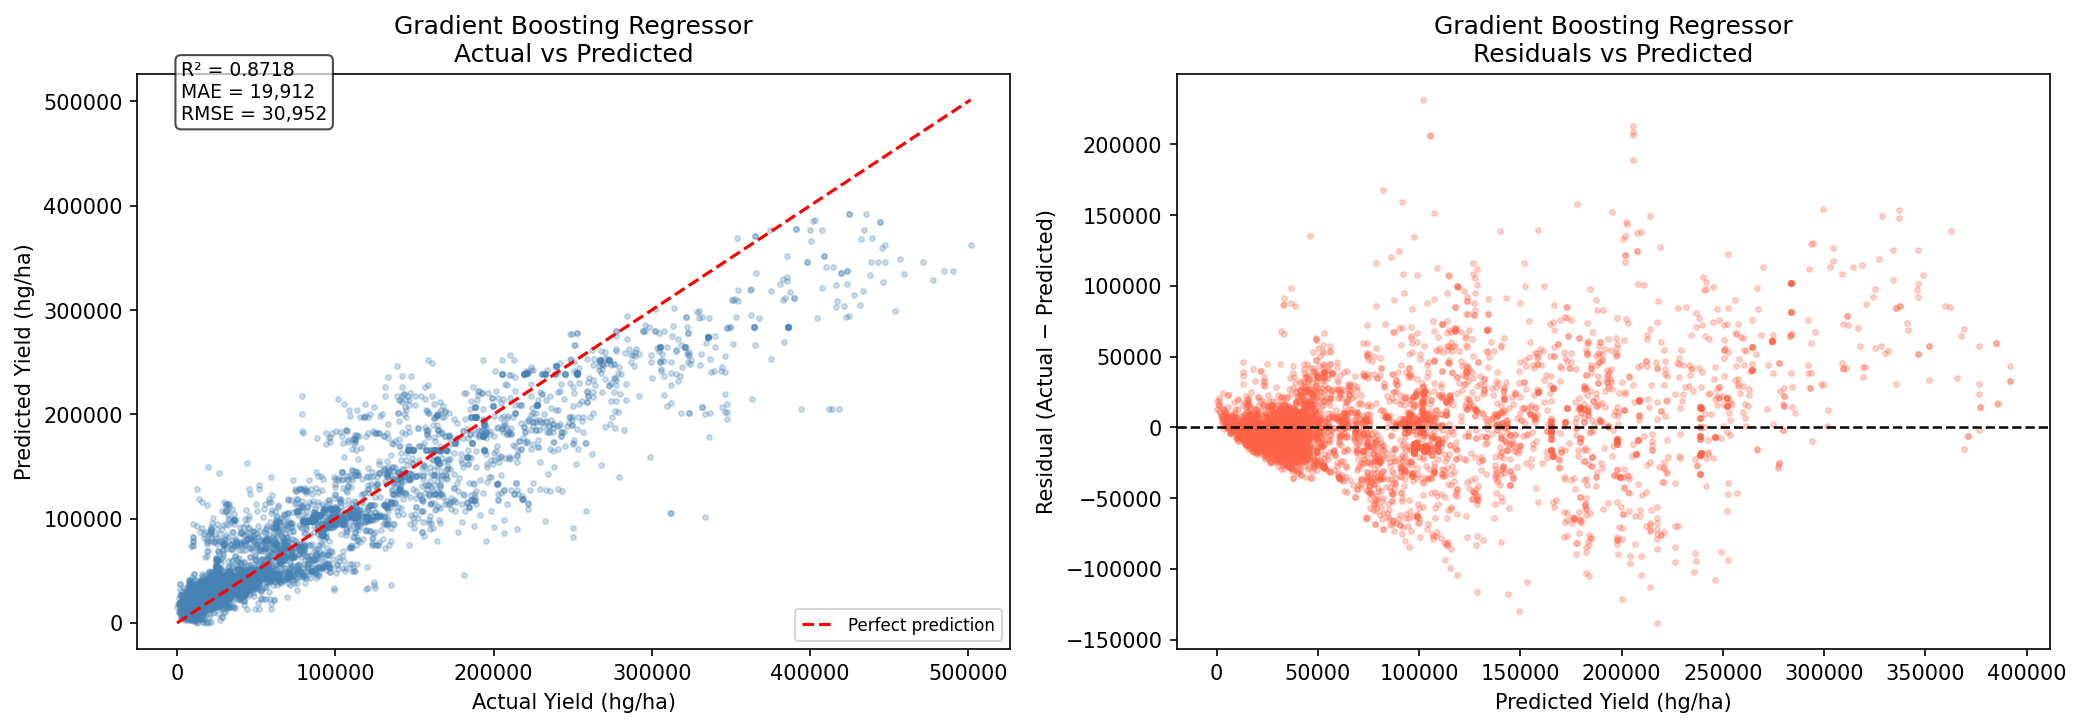
\includegraphics[width=\textwidth]{15_avp_gradient_boosting.png}
  \caption{Gradient Boosting.}
\end{subfigure}

\vspace{4pt}
\begin{subfigure}{0.49\textwidth}
  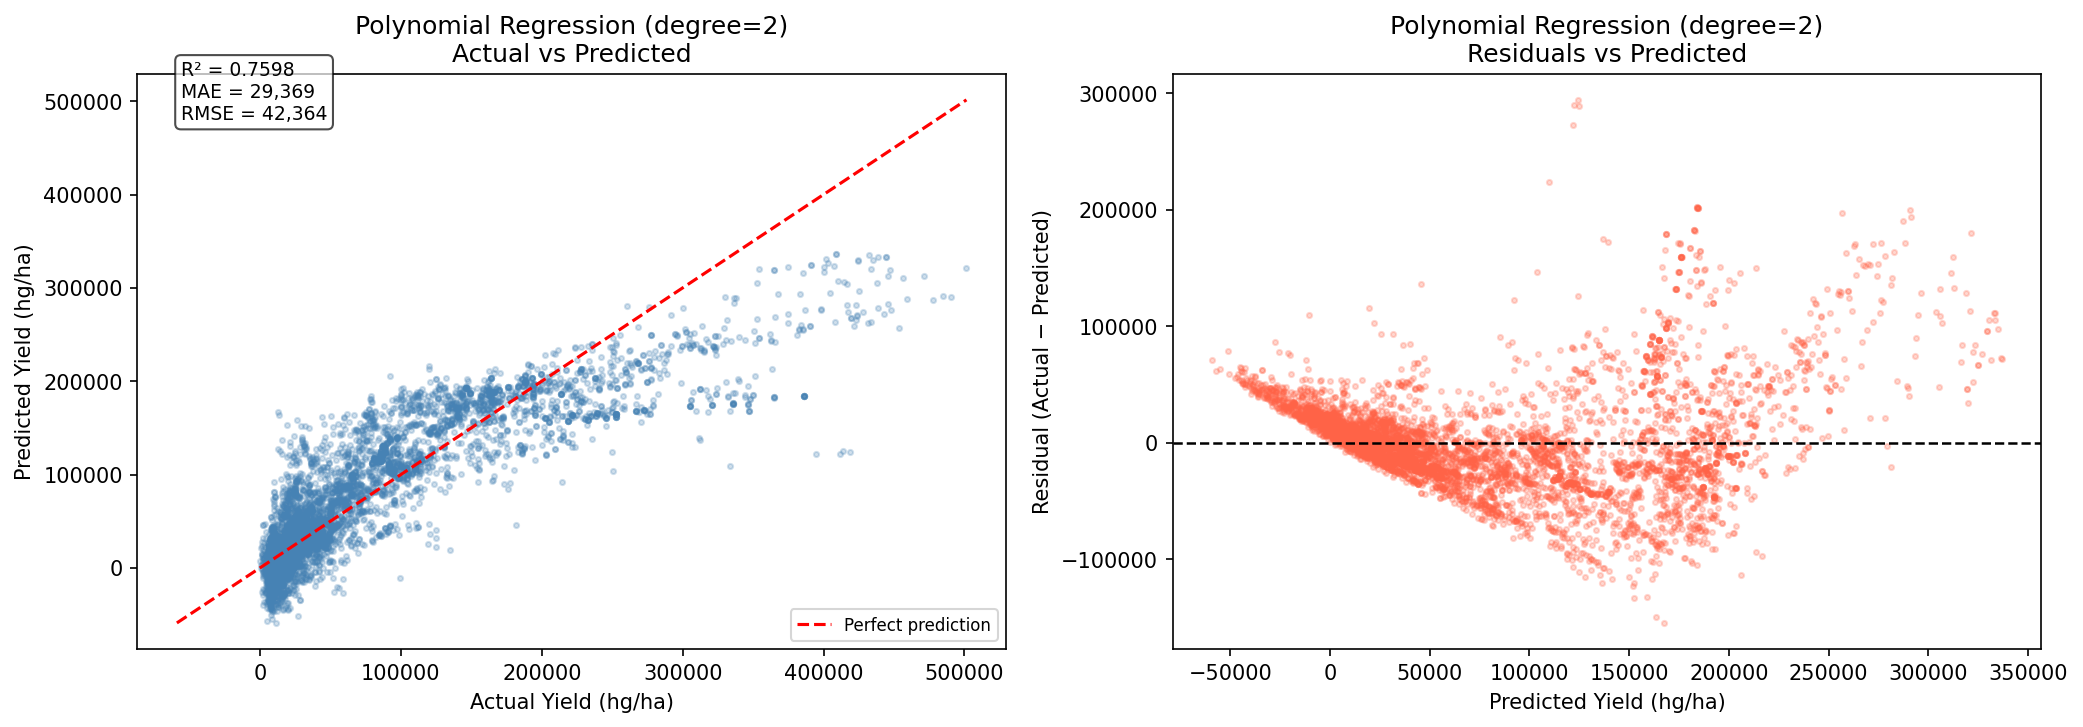
\includegraphics[width=\textwidth]{10_avp_polynomial_deg2.png}
  \caption{Polynomial Regression (deg=2).}
\end{subfigure}\hfill
\begin{subfigure}{0.49\textwidth}
  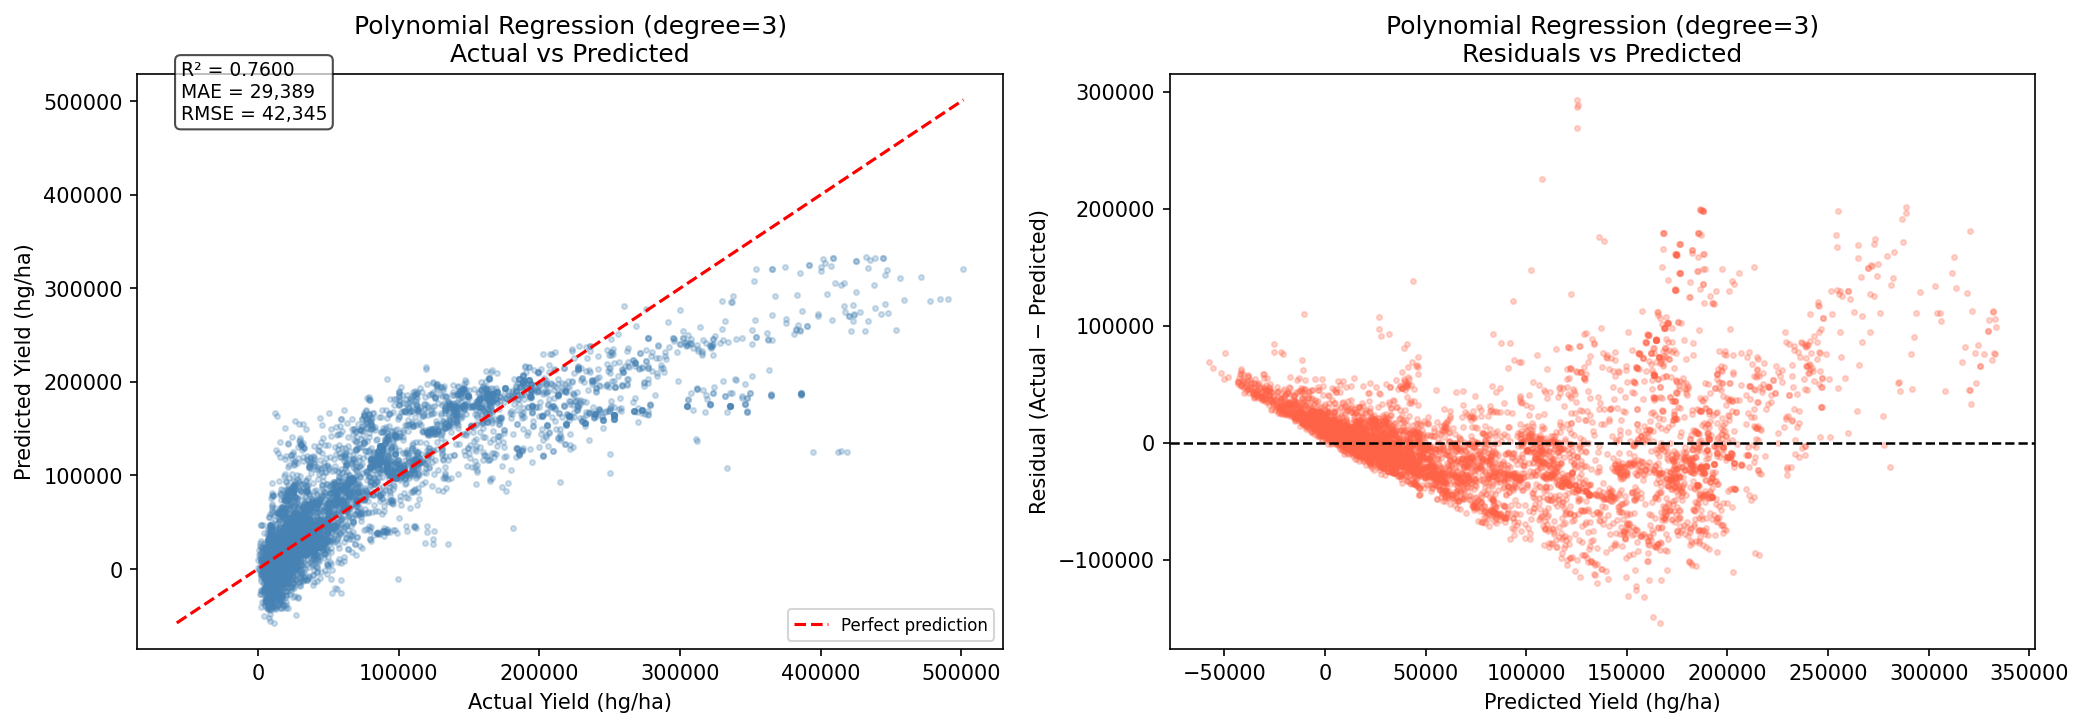
\includegraphics[width=\textwidth]{11_avp_polynomial_deg3.png}
  \caption{Polynomial Regression (deg=3).}
\end{subfigure}

\vspace{4pt}
\begin{subfigure}{0.49\textwidth}
  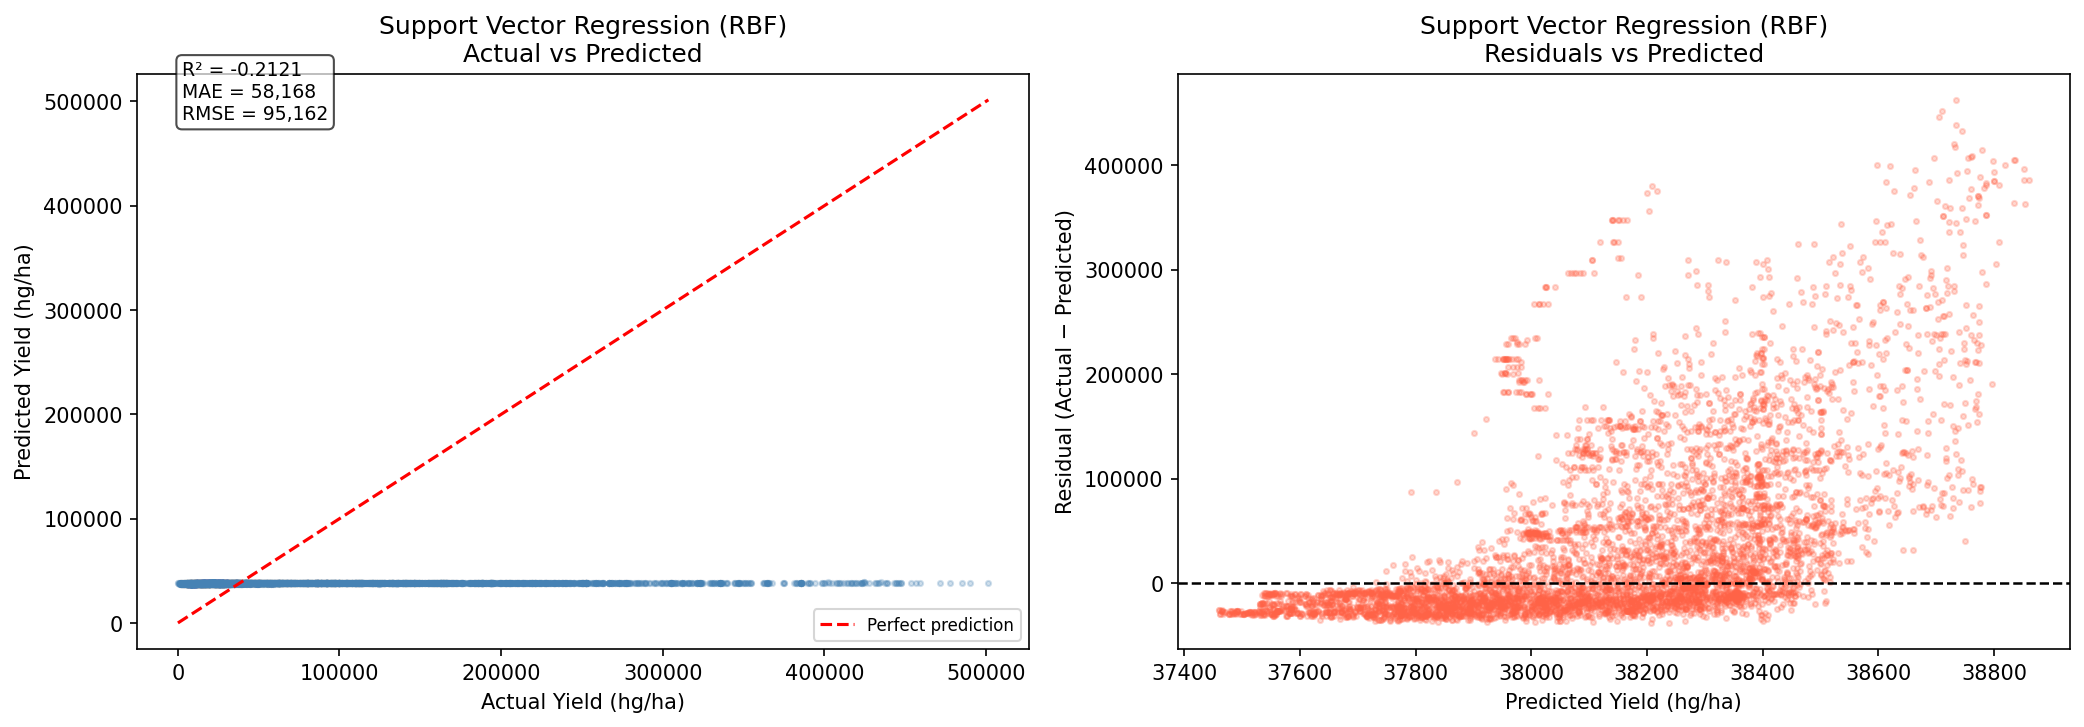
\includegraphics[width=\textwidth]{17_avp_svr.png}
  \caption{SVR (RBF) --- worse than baseline.}
\end{subfigure}
\caption{Actual vs.\ predicted and residual diagnostics per regression model.}
\end{figure}

\paragraph{Discussion.}
The Random Forest explains \textbf{98.9\%} of the variance in yield
($R^2 = 0.9888$) with a mean absolute error of only $\approx$3{,}494~hg/ha ---
a 94.6\% reduction over the baseline. Linear and polynomial models plateau at
$R^2 \approx 0.76$, confirming the non-linear nature of the problem seen in the
EDA. Notably, SVR with an RBF kernel performs \emph{worse than the baseline}
($R^2 = -0.21$): the RBF kernel does not cope well with the sparse,
high-dimensional one-hot encoded feature space.

% ================================================================ 6
\section{Classification Models and Results}\label{sec:clf}

For classification, the continuous yield is discretised. The \textbf{binary}
target splits records at the training mean (77{,}053~hg/ha) into below/above
average. The \textbf{three-class} target uses the 33rd and 67th percentiles to
form low/medium/high bands. Four classifiers were trained for each target:
Random Forest, K-Nearest Neighbors (k=5), Logistic Regression, and Naive Bayes.

\begin{figure}[H]
\centering
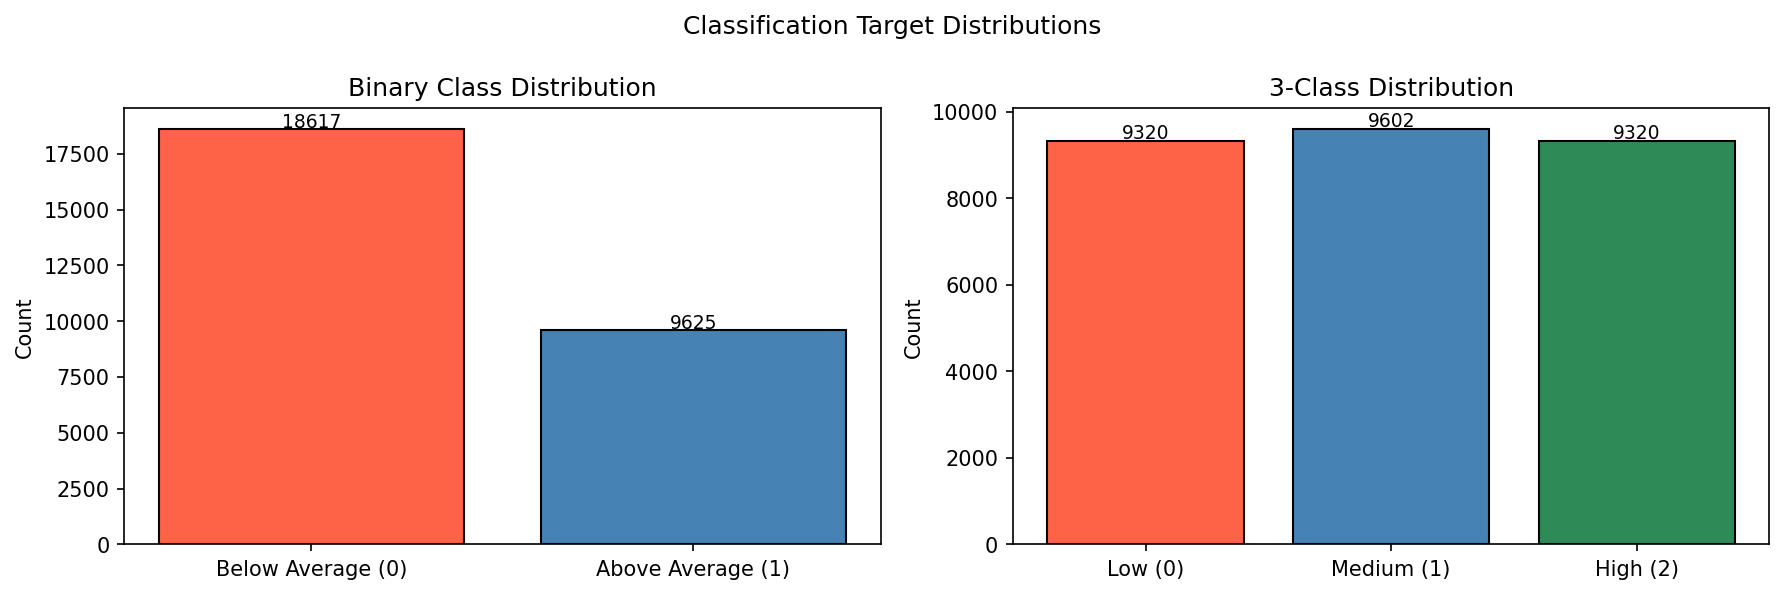
\includegraphics[width=0.9\textwidth]{22_binary_target_distribution.png}
\caption{Class balance for the binary and three-class targets.}
\end{figure}

\subsection{Binary classification}

\begin{figure}[H]
\centering
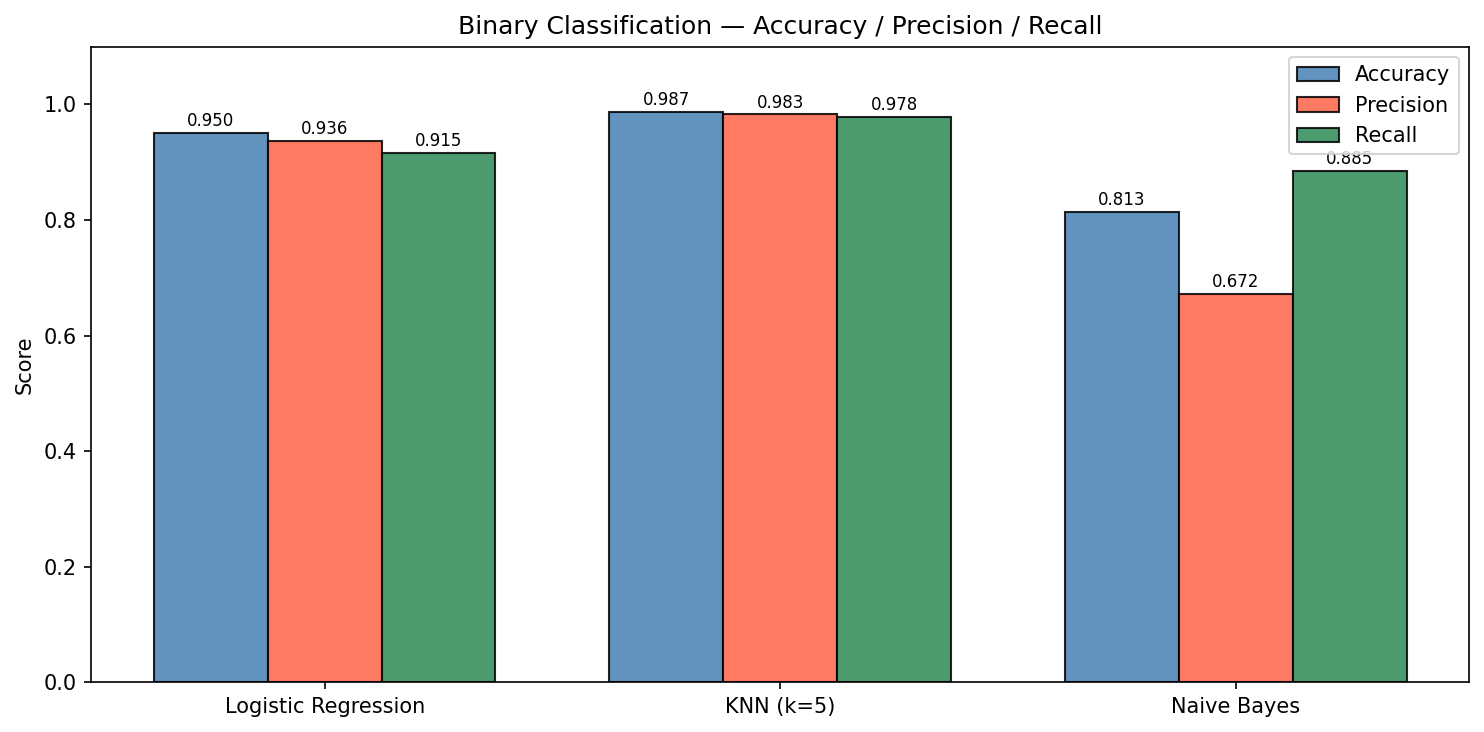
\includegraphics[width=0.95\textwidth]{26_binary_classifiers_comparison.png}
\caption{Binary classification --- accuracy, precision, and recall per model.
KNN achieves the best overall scores.}
\end{figure}

\begin{figure}[H]
\centering
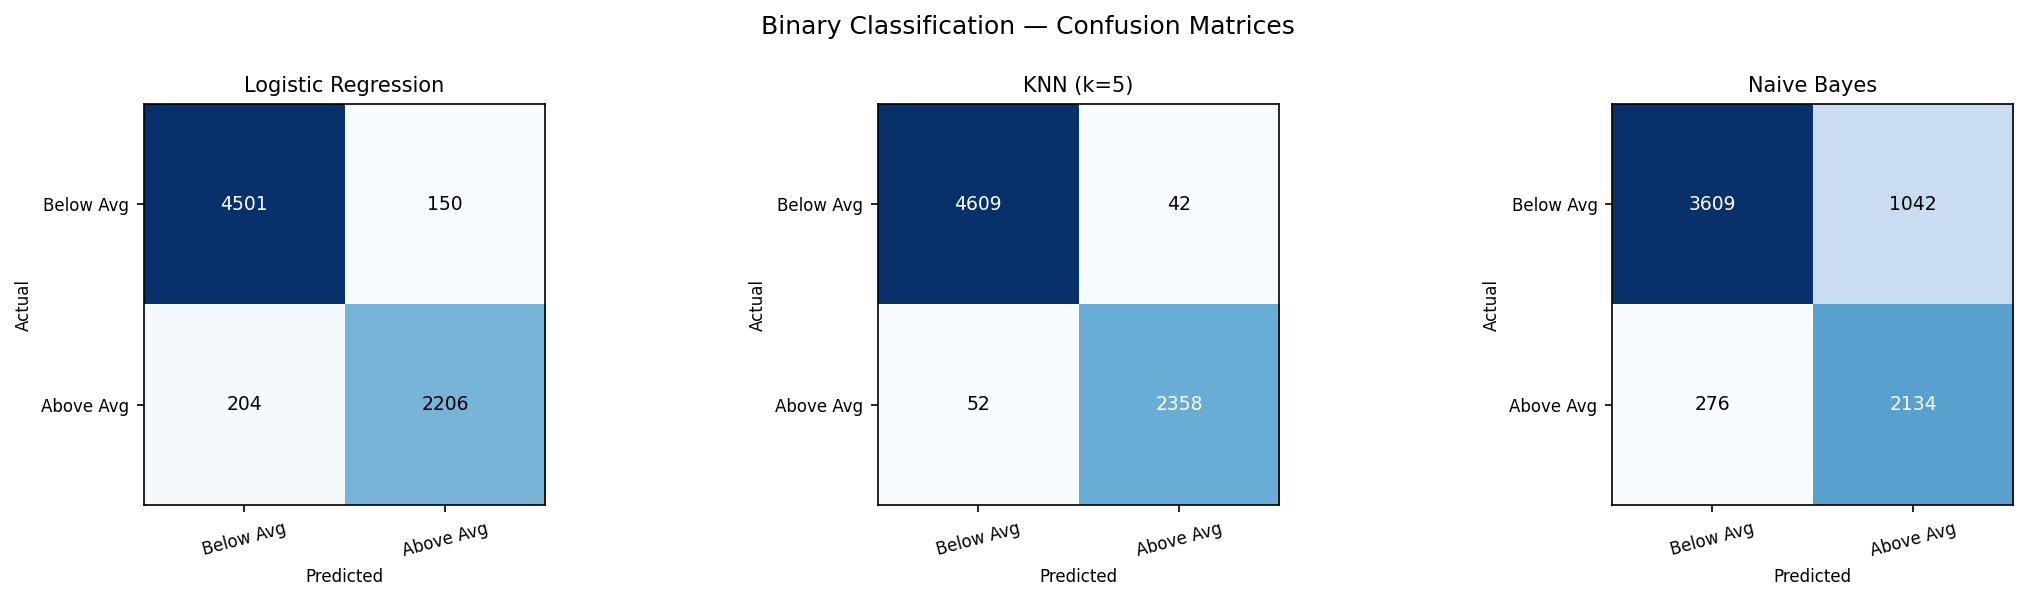
\includegraphics[width=\textwidth]{25b_binary_confusion_matrices_combined.png}
\caption{Confusion matrices for the binary classifiers (Logistic Regression,
KNN, Naive Bayes).}
\end{figure}

\subsection{Three-class classification}

\begin{figure}[H]
\centering
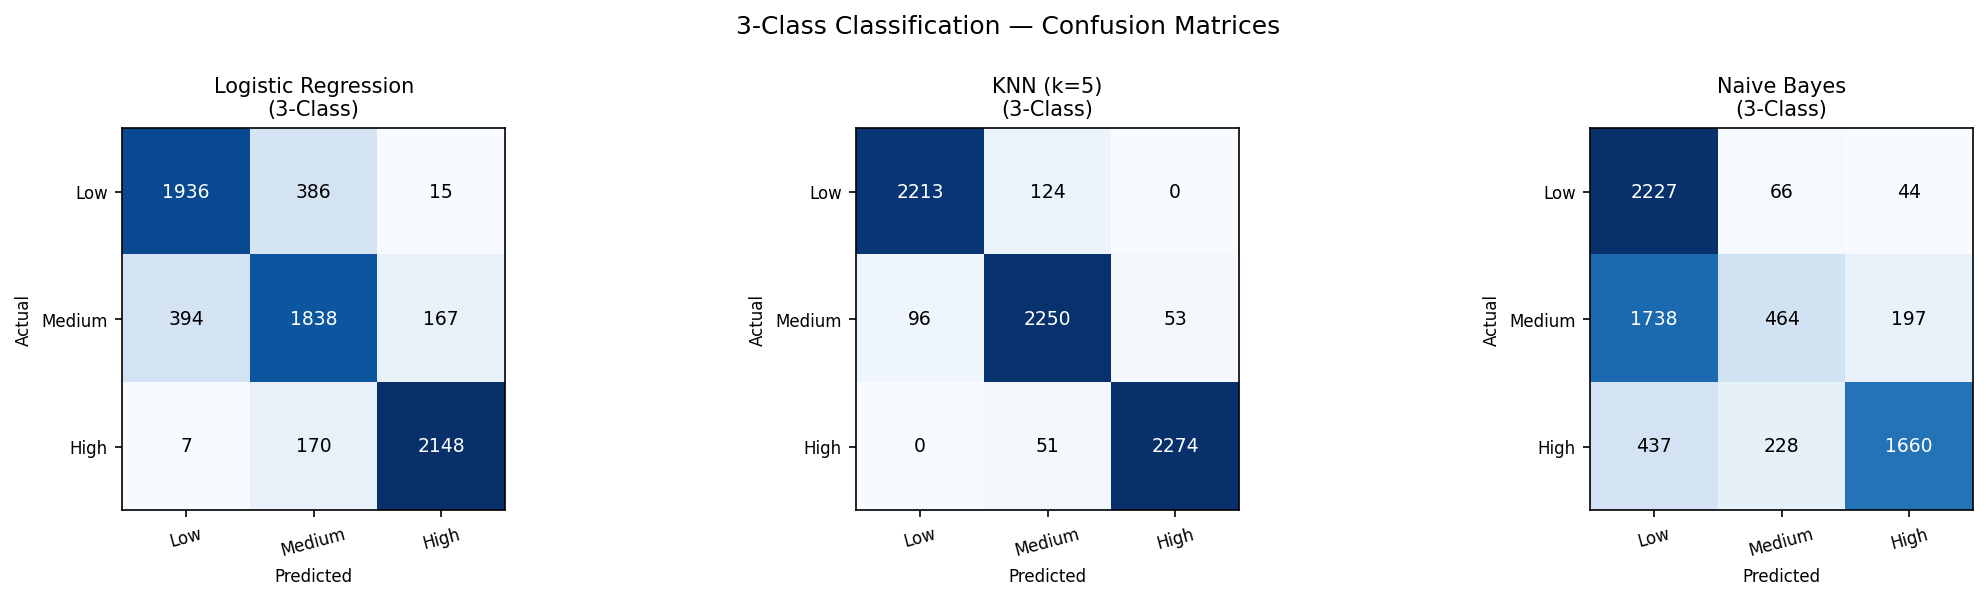
\includegraphics[width=\textwidth]{27_cm_3class.png}
\caption{Confusion matrices for the three-class (low/medium/high) classifiers.}
\end{figure}

\begin{figure}[H]
\centering
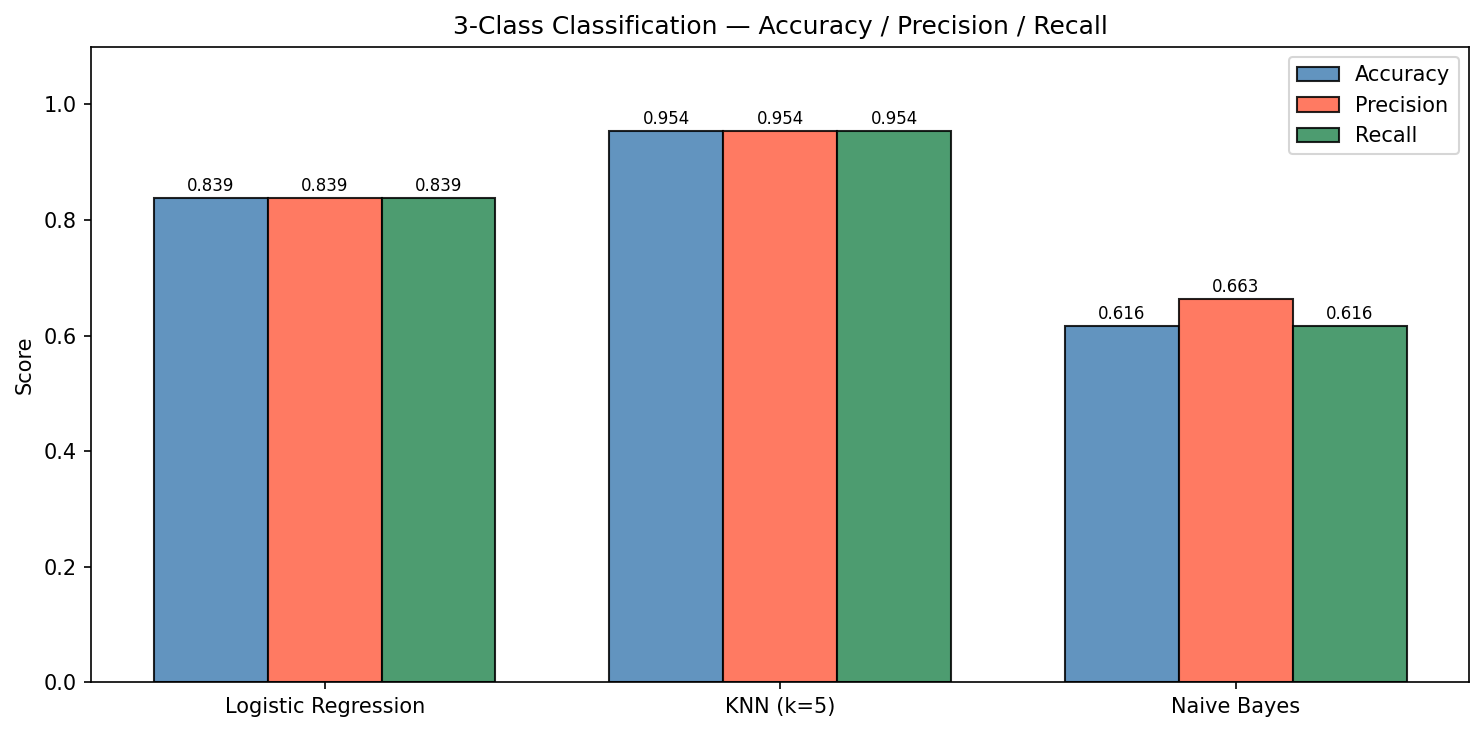
\includegraphics[width=0.95\textwidth]{28_3class_classifiers_comparison.png}
\caption{Three-class classification --- accuracy, precision, and recall per
model.}
\end{figure}

\begin{table}[H]
\centering
\caption{Best classifier per task (accuracy on the test set).}
\begin{tabular}{lll}
\toprule
\textbf{Task} & \textbf{Best model} & \textbf{Accuracy} \\
\midrule
Binary    & K-Nearest Neighbors (k=5) & 0.987 \\
3-class   & K-Nearest Neighbors (k=5) & 0.954 \\
\bottomrule
\end{tabular}
\end{table}

\paragraph{Discussion.}
KNN is the strongest classifier on both targets (binary accuracy 0.987,
three-class accuracy 0.954), narrowly ahead of the Random Forest classifier.
Naive Bayes is the weakest (0.813 binary, 0.616 three-class) because its
assumption of feature independence is violated by the one-hot encoded data.
Interestingly, the best \emph{classifier} (KNN) differs from the best
\emph{regressor} (Random Forest).

% ================================================================ 7
\section{The Application}\label{sec:app}

The project is delivered as an interactive web application (a Flask REST API
serving a React frontend) that covers the full workflow: data exploration,
model benchmarks, visualisations, and live prediction. The dashboard reports the
real dataset statistics and recent predictions.

\begin{figure}[H]
\centering
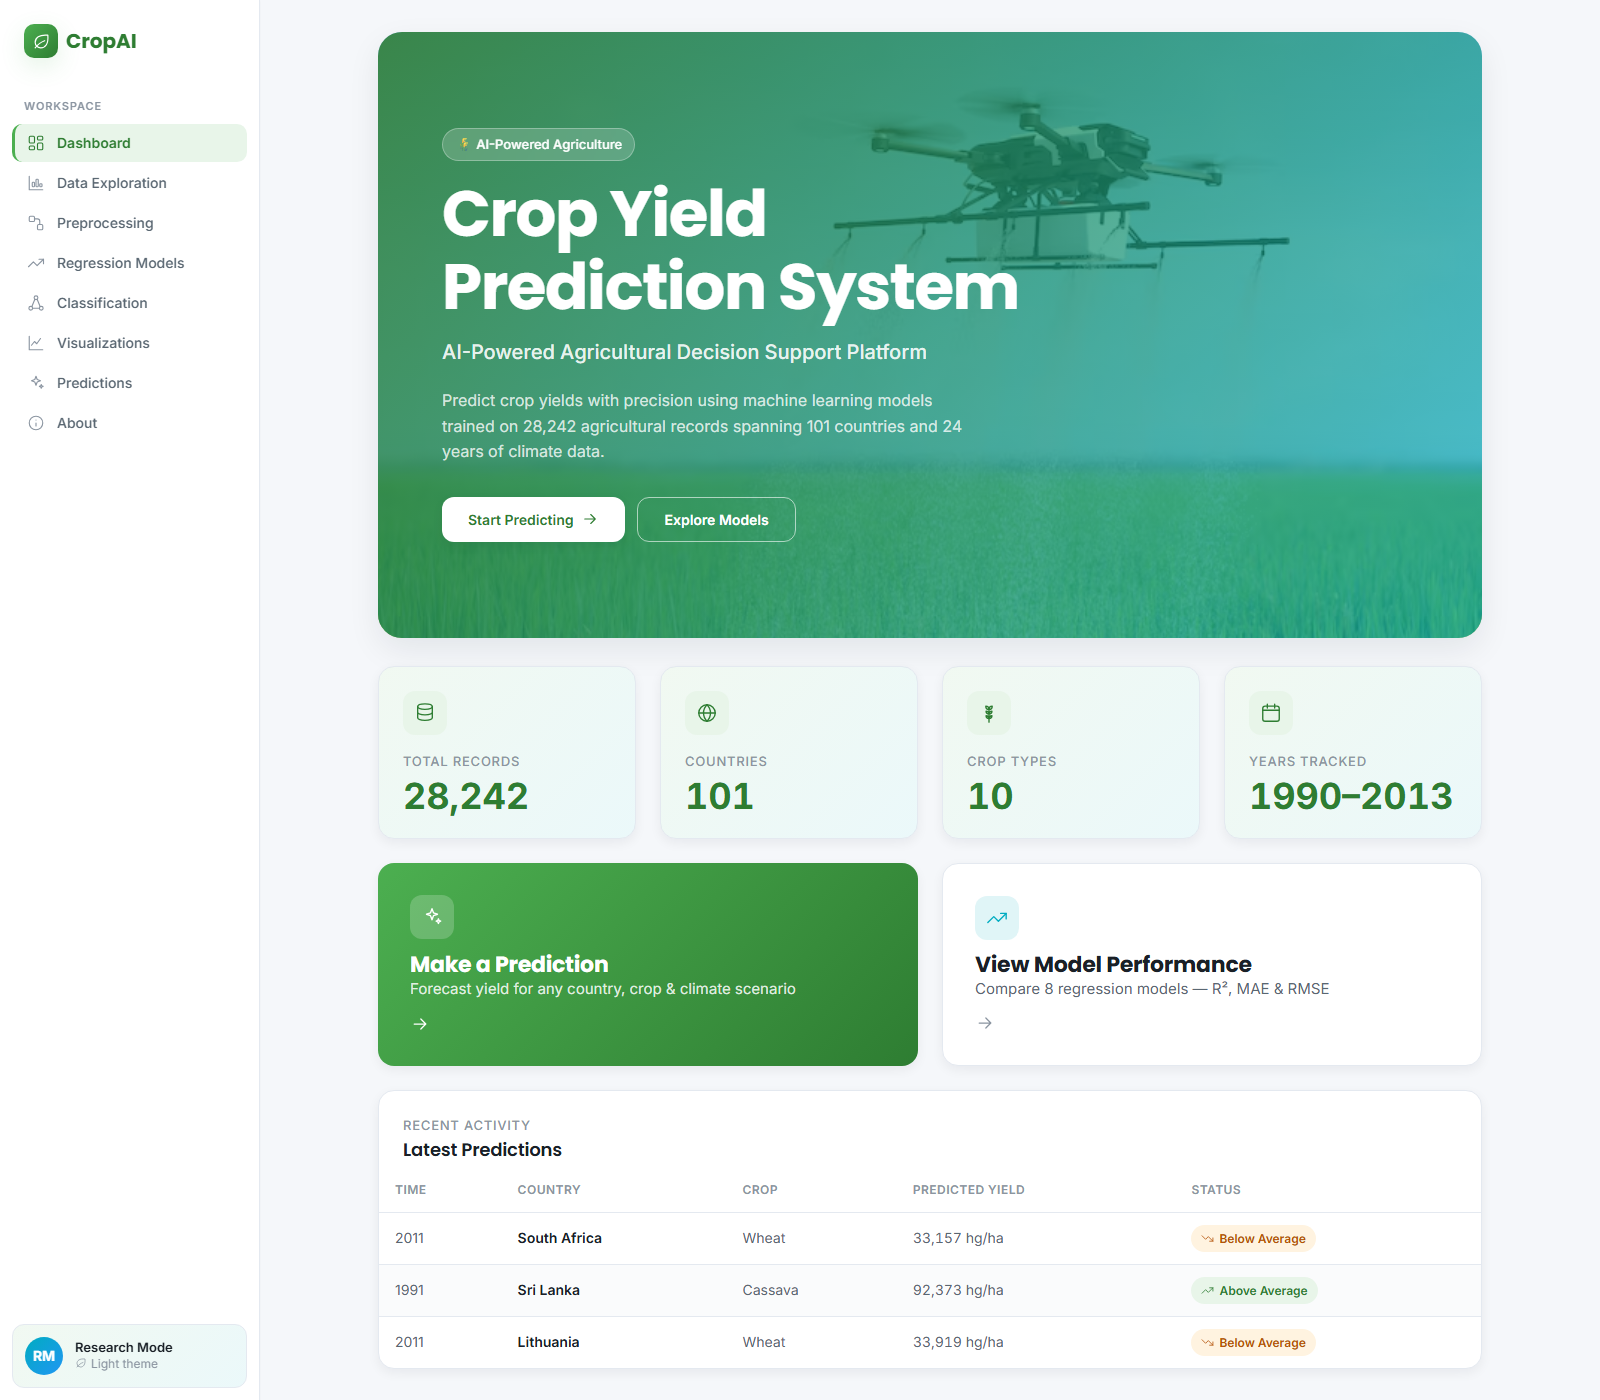
\includegraphics[width=0.8\textwidth]{29_app_dashboard.png}
\caption{The CropAI web application dashboard, showing dataset key figures
(28{,}242 records, 101 countries, 10 crops, 1990--2013), a prediction entry
point, and recent predictions.}
\end{figure}

% ================================================================ 8
\section{Conclusion}\label{sec:conc}

This project built and compared a full suite of supervised models for crop yield
prediction on a 28{,}242-row, 115-feature dataset. The \textbf{Random Forest}
regressor is the best model for predicting exact yield ($R^2 = 0.989$), while
\textbf{KNN} is the best classifier for predicting yield level (98.7\% binary
accuracy). The exploratory analysis and feature-importance results agree that
categorical features (crop and country) carry most of the predictive signal,
and that non-linear ensemble methods substantially outperform linear models and
SVR.

\paragraph{Limitations and future work.}
\begin{itemize}[noitemsep]
  \item The data ends in 2013 and covers only 10 crop types.
  \item The numerical climate features are only weakly correlated with yield;
        adding soil quality, fertiliser, and irrigation data could improve
        accuracy.
  \item Hyperparameter tuning and cross-validation could further refine the
        ensemble models.
\end{itemize}

% ================================================================ refs
\section*{References}
\addcontentsline{toc}{section}{References}
\begin{itemize}[noitemsep]
  \item FAO --- Food and Agriculture Organization of the United Nations,
        crop, pesticide, and climate datasets.
  \item F.\ Pedregosa et al., \emph{scikit-learn: Machine Learning in Python},
        JMLR 12, 2011.
  \item The pandas, NumPy, Matplotlib, and Flask open-source libraries.
\end{itemize}

\end{document}
